% \documentclass[journal, 12pt, onecolumn, draftclsnofoot]{IEEEtran} %JSAC 20'
% \documentclass[sigconf]{acmart} %ACM Mobihoc 20'
% \documentclass[conference]{IEEEtran} %ICDCS 20'
\documentclass[10pt,journal,compsoc]{IEEEtran} %TMC 20'
% \IEEEoverridecommandlockouts
\usepackage[linesnumbered,vlined,ruled]{algorithm2e}
\usepackage{algorithmic}
\usepackage{etoolbox}
\ifCLASSOPTIONcompsoc
  % IEEE Computer Society needs nocompress option
  % requires cite.sty v4.0 or later (November 2003)
  \usepackage[nocompress]{cite}
\else
  % normal IEEE
  \usepackage{cite}
\fi
% \usepackage[noend]{algpseudocode}
\usepackage{graphicx}
\graphicspath{ {./images/} }
\usepackage{amsmath,amsthm,amssymb,amsfonts}
\usepackage{mathtools}
\usepackage[dvipsnames]{xcolor}
\usepackage{dcolumn}
\usepackage[utf8]{inputenc}
\usepackage{soul}
\usepackage{array}
\usepackage{blindtext}
% \renewcommand{\algorithmicforall}{\textbf{for all}}
%---------------------------------------------------------------%
\newtheorem{definition}{Definition}   % 
\theoremstyle{definition}             % alter theorem style: <definition>
\newtheorem{program}{Program}         % [program]
\newtheorem{assumption}{Assumption}   % [assumption]
\newtheorem{example}{Example}         % [example]
\newtheorem{Algorithm}{Algorithm}     % [algorithm]
\newtheorem{policy}{Policy}           % [policy]
\newtheorem{problem}{Problem}         % [problem]
\theoremstyle{remark}                 % alter theorem style: <remark>
\newtheorem{remark}{Remark}           % [remark]
\theoremstyle{plain}                  % alter theorem style: <plain>
\newtheorem{theorem}{Theorem}         % [theorem]
\newtheorem{lemma}{Lemma}             % [lemma]
\newtheorem{corollary}{Corollary}     % [corollary]
%---------------------------------------------------------------%
\newcommand{\eq}{=}
\newcommand{\domZ}{\mathbb{Z}_{*}}
\newcommand{\domP}{\mathbb{Z}_{*}}
\newcommand{\vecOne}{\mathbf{1}}
\newcommand{\ind}{\mathbf{I}}
\newcommand{\mat}{\mathbf}
\newcommand{\Poisson}{\text{Poisson}}
\newcommand{\Bernoulli}{\text{Bernoulli}}
\newcommand{\define}{\triangleq}
\newcommand{\leadto}{\Rightarrow}
\newcommand{\vecG}{\boldsymbol}
\renewcommand{\vec}{\mathbf}
\DeclarePairedDelimiter{\set}{\{}{\}}
\DeclarePairedDelimiter{\norm}{|}{|}
\DeclarePairedDelimiter{\Inorm}{\|}{\|_1}
\DeclarePairedDelimiter{\Paren}{\bigg(}{\bigg)}
\DeclarePairedDelimiter{\Bracket}{\bigg[}{\bigg]}
\DeclarePairedDelimiter{\Brace}{\bigg\{}{\bigg\}}
%---------------------------------------------------------------%
\newcommand{\fixit}[1]{{\leavevmode\color{red}#1}}
\newcommand{\comments}[1]{{\leavevmode\color{blue}#1}}
\newcommand{\accept}[1]{#1}
\newcommand{\deny}[1]{}
\newcommand{\delete}[2]{}
\newcommand{\needref}[1]{\text{[#1]}}
%---------------------------------------------------------------%
\newcommand{\AP}{\dagger}
\newcommand{\ES}{\ddagger}
\newcommand{\apSet}{\mathcal{K}}
\newcommand{\esSet}{\mathcal{M}}
\newcommand{\ccSet}{\mathcal{X}}
\newcommand{\jSpace}{\mathcal{J}}
\newcommand{\Stat}{\mathbf{S}}
\newcommand{\Obsv}{\mathcal{Y}}
\newcommand{\Policy}{\vecG{\Omega}}
\newcommand{\Delay}{\vecG{\mathcal{D}}}
\newcommand{\Baseline}{\vecG{\Pi}}
\newcommand{\algname}{Solver}

\newcommand{\wangr}[1]{{\leavevmode\color{orange}#1}}
\newcommand{\hongyc}[1]{{\leavevmode\color{purple}#1}}
\newcommand{\tann}[1]{{\leavevmode\color{blue}#1}}
%---------------------------------------------------------------%
\newcommand{\brlatency}{signaling latency}

%---------------------------------------------------------------%
\def\BibTeX{{\rm B\kern-.05em{\sc i\kern-.025em b}\kern-.08em
    T\kern-.1667em\lower.7ex\hbox{E}\kern-.125emX}}
%---------------------------------------------------------------%

\begin{document}
    \title{Distributed Job Dispatching in Edge Computing Networks with Random Uploading Latency: A Low-Complexity POMDP Approach
    }

    \author{
        Yuncong~Hong,%~\IEEEmembership{Student Member,~IEEE,}
        Bojie~Lv,%~\IEEEmembership{Student Member,~IEEE,}
        Rui~Wang,%~\IEEEmembership{Member,~IEEE,}
        Haisheng~Tan,%~\IEEEmembership{Senior Member,~IEEE,}
        Zhenhua~Han,%~\IEEEmembership{Member,~IEEE,}
        and~Francis~C.M.~Lau%~\IEEEmembership{Member,~IEEE,}
    }%
    % \author{
    %     \IEEEauthorblockN{
    %         Yuncong Hong\IEEEauthorrefmark{1}\IEEEauthorrefmark{2},
    %         Bojie Lv\IEEEauthorrefmark{1},
    %         Rui Wang\IEEEauthorrefmark{1},
    %         Haisheng Tan\IEEEauthorrefmark{3},
    %         Zhenhua Han\IEEEauthorrefmark{2},
    %         Francis C.M. Lau\IEEEauthorrefmark{2}
    %     }
    %     \IEEEauthorblockA{\IEEEauthorrefmark{1}
    %         Department of Electrical and Electronic Engineering, Southern University of Science and Technology, Shenzhen, China \\
    %     }
    %     \IEEEauthorblockA{\IEEEauthorrefmark{2}
    %         Department of Computer Science, The University of Hong Kong, Hong Kong, China \\
    %     }
    %     \IEEEauthorblockA{\IEEEauthorrefmark{3}
    %        LINKE Lab, University of Science and Technology of China, Hefei, China \\
    %     }
    % }
    % \thanks{Manuscript received April 19, 2005; revised August 26, 2015.}}

    % \markboth{Journal of \LaTeX\ Class Files,~Vol.~14, No.~8, August~2015}%
    % {Shell \MakeLowercase{\textit{et al.}}: Bare Demo of IEEEtran.cls for Computer Society Journals}

    \IEEEtitleabstractindextext{
    \begin{abstract}
        %NOTE: (1) random latency matters; why random latency matters;
        Random transmission latency is appeared as a non-negligible issue in edge computing system when considering distributed scheduler implementation in a large network such as Metropolitan Area Network (MAN).
        With the random latency of information sharing among distributed schedulers, the shared system status information would inevitably become stale and thus deviates the optimality. %drift away from optimality.
        %NOTE: (2) online/distributed/cooperative/job dispatching/outdated information
        In this paper, we investigate an online distributed cooperative job dispatching problem in an edge computing system residing in a MAN, where multiple access points (APs) collect jobs from the mobile users and upload each job to one edge server for computation.
        %NOTE: (3) the signaling (information sharing) mechanism; partial information reception
        % we design the broadcast mechanism and extend to a general partial information practice with partial information, in the distributed system design.
        Furthermore, we introduce a signaling mechanism to facilitate information sharing among distributed schedulers on each AP.
        % with periodic broadcast to facilitate cooperations among APs.
        Moreover, the fully-observed system state is discouraged as reception of all broadcast is time consuming.
        The signaling and job dispatching latency is random and non-negligible in MAN, and the APs have to update their job dispatching strategies according to partially received and outdated broadcast information.
        %NOTE: (4) technical contribution: we leverage POMDP to formulate this {long-term dynamic} problem, and design a {delicate} low-complexity framework, and extend it to unknown-priori scenario via a novel reinforcement learning framework.
        We formulate the distributed optimization of job dispatching strategies at all the APs, with partial and outdated information, as a partially observable Markov decision process (POMDP).
        %whose minimization objective is a discounted measurement of job delivery and computation time.
        % The conventional solution for POMDP is impractical due to huge time complexity.
        % In this paper, we propose a novel low-complexity solution framework for distributed job dispatching.
        % Based on it, the optimization of job dispatching policy can be decoupled via an \emph{alternative policy iteration algorithm}, called \algname, so that the distributed policy iteration of each AP can be made according to partial and outdated observation.
        % An analytical performance lower bound is provided for the approximate MDP solution.
        Furthermore, we extend \algname~to handle a more general scenario where the statistics of job arrivals, uploading latency and job processing time are unknown.
        The extended \algname~leverages a novel and efficient reinforcement learning approach to online continuously improve the system performance.
        % NOTE: (5) the simulation and performance improvement
        % Finally, we conduct extensive simulations based on the Google Cluster trace.
        % The evaluation results show that our policy can achieve as high as $20.67\%$ reduction in average job response time compared with heuristic baselines, and our algorithm consistently performs well under various parameter settings.
    \end{abstract}

    % Note that keywords are not normally used for peer-review papers.
    \begin{IEEEkeywords}
        Edge computing, metropolitan area network, partially-observable MDP, reinforcement learning.
    \end{IEEEkeywords}
}

    \maketitle
    
    
\IEEEraisesectionheading{
    \section{Introduction}
    \label{sec:introduction}
}
%NOTE: General Background of MEC and Motivation
\IEEEPARstart{E}{dge} computing is a promising solution for increasing computation-intensive and energy-hungry applications on mobile devices.
Large amount of mobile devices can connect to the access points (APs) which functions as gateway to aggregate and dispatch jobs to the edge servers \cite{MEC-SURVEY}.
The edge servers are deployed in closer proximity to APs than cloud infrastructure, which alleviate the communication overhead and enable computation of time-sensitive jobs.
However, the edge servers are always deployed with limited computation resources.
The establishment of efficient cooperation among edge servers is one of the major design challenges, \comments{given the signaling overhead introduced in signaling mechanism design.}
%given the network transmission latency and signaling overhead

%NOTE: Motivation with MAN
We consider an edge computing system with multiple APs and edge servers residing in the Metropolitan Area Network (MAN).
The APs should collect jobs offloaded from the mobile users in its service area and make dispatching decisions for each job.
\comments{
    The existing literature, such as \cite{tan-online,MOBIHOC19-ZhouZ,IOTJ18-FanQ,TOC19-LiuC,JSAC19-AlameddineHA}, usually assumed that the transmission latency cause of job offloading is non-negligible and fixed in the edge computing network.
    Moreover, it would cause big problem with job dispatching decision making with random signaling overhead (because no work considering the practical dispatcher design).
    In the following literature \cite{TWC18-LyuX,latency-EDGE19}, the network transmission latency could be fluctuate in such extensive network.
}
However, according to the MAN performance analysis research in \cite{MAN-LATENCY}, the transmission latency will vary a lot with respect to different hours of day and devices' locations in a MAN.
This brings new challenges to the job dispatcher design in the edge computing network.
Firstly, the centralized dispatcher design is discouraged for outdated system information and unpredictable signaling latency.
Secondly, the cooperation of distributed dispatchers suffers from significant signaling overhead, and the random transmission latency causes the inconsistency of system information at different dispatchers.

%NOTE: Our contributions
In this paper, we would like to shed some lights on the above challenging distributed dispatcher design via POMDP problem formulation and a novel low-complexity approximate MDP solution framework.
Specifically, the signaling latency among APs and edge servers and job uploading latency from APs to edge servers are assumed to be random, and hence each AP can only observe part of the system state with random latency.
Our contributions in this new optimization scenario are summarized as follows.
\begin{itemize}
    \item We propose a novel low-complexity distributed solution framework for the dispatcher design at the APs, where each AP collects the information only from the APs and edge servers in a close proximity and make dispatching decisions with random signaling latency. We directly derive the expression of approximate value function and obtain distributed dispatching policy via alternative policy iteration. Thus, the complicated POMDP solution or value iteration is avoided. To our best knowledge, this is the first work to address the cooperative distributed multi-agent optimization problem under MDP framework.
    \item We derive an analytical cost lower bound for the proposed distributed dispatching policy in the above novel solution framework. In the conventional approximate MDP method, the performance is usually evaluated via numerical method, and it is hard to obtain analytical performance bound.
\end{itemize}

The remainder of this paper is organized as follows.
In Section \ref{sec:review}, the related works are elaborated.
In Section \ref{sec:model}, we illustrate the system model and the signaling model with random latency.
In Section \ref{sec:formulation}, we formulate the global optimization of dispatching decisions at all APs as an POMDP.
In Section \ref{sec:algorithm}, we introduce the novel low-complexity distributed solution framework for the above POMDP.
The numerical analysis of the proposed solution is provided in Section \ref{sec:evaluation}, and the conclusion is drawn in Section \ref{sec:conclusion}.

\section{Related Works}
\label{sec:review}
%NOTE: resource placement (cache-like problem), service migration
There have been a number of works focusing on the resource allocation, job dispatching and service migration of edge computing system.
For example, in \cite{TON19-WangSq}, the edge servers are one-to-one bound to the base stations (BSs), and the job migration could be applied according to users' mobility traces via the backhaul network connecting the BSs.
However, according to a recent research \cite{INFOCOM19-WuC}, the resource re-allocation for running jobs on servers is hard to implement in practice, as it's hard for jobs migration among heterogeneous edge servers with different resource configurations.
Hence, it might be more important to optimize the job dispatching strategy at their arrival time.

%NOTE: single-agent dispatching, single UE/server
There also have been a number of works considering the centralized job dispatching with instant and complete knowledge on the states of edge computing systems. For example, in order to minimize the average job response time in the worst case, the authors in \cite{tan-online} designed an online algorithm for job dispatching in edge computing systems with fixed uploading latency. In the scenario that BSs and edge servers are connected via software defined network (SDN), the authors in \cite{IOTJ18-FanQ} proposed a heuristic algorithm to dispatch the jobs to the closest edge servers according to geographical locations. When the jobs can be dispatched to either edge servers or cloud servers with fixed uploading latency, the authors in \cite{MASS18-MengZ} formulated job dispatching problem as an integer linear programming to minimize the total uploading latency.
In the above works, a centralized dispatcher with complete and instant knowledge of the system status is assumed in the edge computing systems, which might be impractical.

Hence, there are also some works considering the distributed job dispatching in edge computing systems. For example, in order to minimize a weighted sum of total energy consumption and uploading latency, the authors in \cite{ToN-Xuchen2016} proposed a distributed job dispatching algorithm based on game theory to achieve the Nash equilibrium. 
Considering job migration at edge servers, the authors in \cite{ToN-xujie2018} optimized the edge computing performance in a distributed manner with limited energy resources via a congestion game framework.
However, in the above works, the latency of information exchange among APs and edge servers is ignored.
In fact, due to the complicated network traffic, this latency might be significant, and the staleness of system state information at the dispatcher of a edge computing systems should be considered.

%NOTE: stale-information based multi-agent related works
The staleness of information sharing among APs and edge servers may degrade the performance of the job dispatching algorithm in edge computing systems.
To the best of our knowledge, there are very limited works investigating this issue.
For example, the authors in \cite{JSAC17-LyuX} proposed a randomized policy via Lyapunov optimization approach to stabilize the queues in a MEC system with multiple IoT devices offloading jobs to one edge server, where \brlatency~is considered. 
In \cite{TWC18-LyuX}, the above approach is applied to the scenario that mobile devices offload jobs to each others via D2D link.
In the above two works, there is one centralized dispatcher in the system and the objective is to stabilize the transmission queues.
Hence, the existence of \brlatency~may not raise significant challenge to the algorithm design with Lyapunov optimization.
However, the design of distributed dispatchers with \brlatency~could be more challenging.
For example, the signaling latencies at distributed dispatchers could be different, and the synchronization of them become infeasible.
Furthermore, it is of more practical significance favor for the distributed dispatchers to make scheduling decisions based on locally observed system state information, instead of global state information.
To our best knowledge, there is no appropriate optimization framework for the distributed dispatcher design with both \brlatency~and partially observable system state information to date.

%----------------------------------------------------------------------------------------%

    % \input{src/02a-background}
    % \section{Motivation}

\begin{enumerate}
    \item Why it's important to consider information latency to dispatching decision making (kind of AoI but periodic).
    \item Support material for stochastic latency and why is neglected.
\end{enumerate}

    \section{System Model}
\label{sec:model}
In this section, we elaborate the model of edge computing networks with random job arrivals, uploading latency and computation time, as well as the signaling mechanism with periodic broadcast.
% as well as the signaling model with periodic broadcast which introduce the job dispatching actions making under partially observable system state at each AP.
%----------------------------------------------------------------------------------------%
\subsection{Network Model}
% \begin{figure*}[htp!]
%     \centering
%     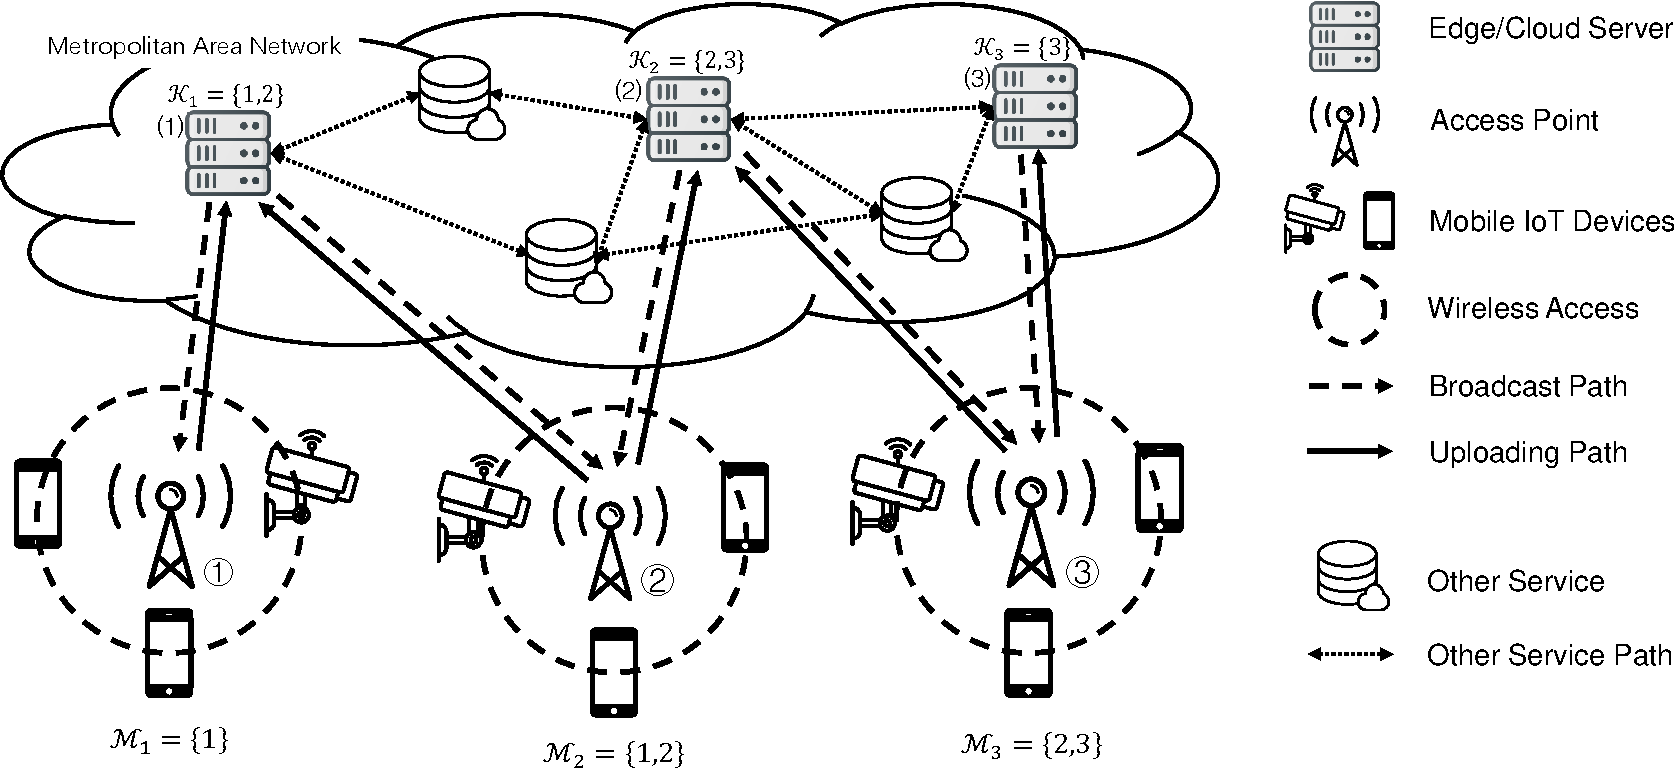
\includegraphics[width=0.60\textwidth]{system-model.pdf}
%     \caption{The Illustration of System Model.}
%     \label{fig:system}
% \end{figure*}
We consider an edge computing system with $K$ Access Points (APs) and $M$ edge servers, which are connected in an edge network as illustrated in Fig.\ref{fig:system}.
The sets of APs and edge servers are denoted as $\apSet \define \set{1,\dots,K}$ and $\esSet \define \set{1,\dots,M}$, respectively.
\hongycCHK{An edge server is typically deployed and collocated with an AP so that mobile devices can upload jobs efficiently.} 
% The communication latency among these APs and edge servers is random.
Each AP collects the computation jobs from the {mobile IoT devices} within its coverage, and makes dispatching \revision{decisions} on the edge servers for each job.
It is assumed that the $k$-th AP only dispatches the computation jobs to the edge servers within a certain number of hops.
Let $\esSet_{k} \subseteq \esSet$ be the subset of edge servers which can compute the jobs from the $k$-th AP, and $\apSet_{m}$ be the subset of APs, which may upload jobs to the $m$-th edge server.
We refer to $\esSet_{k}$ as the \emph{candidate server set} of the $k$-th AP, $\apSet_{m}$ as the \emph{potential AP set} of the $m$-th edge server, \hongycCHK{and $\rho_{k,m}$ as the collocation indicator (i.e., $\rho_{k,m}=1$ if $k$-th AP and $m$-th edge server collocated, otherwise $\rho_{k,m}=0$)} ($\forall k\in\apSet, m\in\esSet$).
Different APs may have different candidate servers according to their locations in the network.%, as illustrated in Fig.\ref{fig:system}.
In this edge computing network, APs and edge servers periodically broadcast their state information (the state information is defined in Section \ref{subsec:broadcast}), and one AP updates its strategy of job dispatching when receiving the broadcast state information.
In this paper, we shall optimize the job dispatching strategy distributed at APs with partially observable state information, where both job uploading and state information broadcasting suffer from random transmission latency.

%NOTE: [job space support and arrival process]
Without loss of generality, it is assumed that there are $J$ types of jobs in this system, which are denoted via the set $\jSpace \define \set{1,\dots,J}$.
The time axis of dispatching is organized by time slots.
The arrivals of the type-$j$ jobs at the $k$-th AP ($\forall k\in\apSet,j\in\jSpace$) in different time slots are assumed to be independent and identically distributed (i.i.d.) Bernoulli random variables, and the arrival probability is denoted as $\lambda_{k,j}$.
Let $B_{k,j}(t) \in \set{0,1}$ represent the event of job arrival, where $B_{k,j}(t)=1$ means one type-$j$ job arrives at the $k$-th AP in the $t$-th time slot, and $B_{k,j}(t)=0$ means otherwise.
Hence,
\begin{align}
    \Pr\{ B_{k,j}(t) = 1 \} = \lambda_{k,j}, \forall t,k\in\apSet,j\in\jSpace.
\end{align}

%NOTE: [uploading process]
Each AP immediately dispatches each type of received jobs to one edge server.
As the APs upload jobs over shared edge networks illustrated in Fig.\ref{fig:system}, the actual uploading time is random due to random traffics initiated from other enabled services.
Moreover, the notification of uploading completion from edge server to AP also consumes random time slots for the same reason, and thus the uploading time is unknown in advance.
Hence, we assume the uploading time of different types of jobs from different APs to edge servers follow independent and discrete distributions.
% \fixit{For the uploading latency of the type-$j$ job from the $k$-th AP to the $m$-th edge server, the other jobs in uploading could be taken as random traffics of other services, and thus the random uploading latency are independent for each job.}
% Different types of jobs may have different distributions of the input data size.
Let $\mathbb{U}_{k,m,j}(\Xi)$ be the uploading latency (in terms of time slots) distribution of the type-$j$ jobs from the $k$-th AP to the $m$-th edge server with support $\set{1, \dots, \Xi}$ ($\forall k\in\apSet, m\in\esSet, j\in\jSpace$), where $\Xi$ is the maximum possible uploading time for all jobs and the expectation is denoted as $u_{k,m,j}$.
\hongycCHK{Specifically, the uploading latency is fixed as $0$ if $\rho_{k,m}=1$ for job uploading to the collocated edge server.}

%NOTE: [computation process]
For job computation process on edge servers, we adopt the \emph{unrelated machines assumption} as in \cite{tan-online} where the computation time on different edge servers would follow independent distributions.
Specifically, there are $J$ parallel virtual machines (VMs) running on each edge server for processing the $J$ job types, respectively.
It is assumed that the computation time of different job types on different edge servers follows independent memoryless geometric distribution 
\footnote{In this paper, we adopt the memoryless geometric distribution to simplify the elaboration of algorithm. In fact, the proposed algorithm can be easily extended to other distributions.}
with different expectations as in \cite{TOWC18-HuangKb}.
Let $\mathbb{G}(1/c_{m,j})$ be the distribution of the computation time slots for the type-$j$ jobs on the $m$-th edge server, where $\mathbb{G}$ denotes the geometric distribution, $c_{m,j}$ is the expectation.
Let $f_{m,j}$ be its probability mass function (PMF), we have
\begin{align}
    f_{m,j}(x) \define (1-\frac{1}{c_{m,j}})^{x-1} \frac{1}{c_{m,j}}, x=1,2,\dots.
\end{align}
For each job type, the uploaded jobs are computed in a First-Come-First-Serve (FCFS) manner, and a processing queue with a maximum job number $L_{max}$ is established for each VM.
The arrival jobs will be discarded when the processing queue is full.

\begin{remark}%[Generalization to Edge-Cloud Model]
    The above network model could be generalized into \revision{a} computing system with both edge servers and cloud center.
    A cloud center could be treated as a special edge server in our model but with stronger computational capability and larger uploading latency and signaling latency \tannCHK{to the APs}.
    % Furthermore, the placement of edge servers in the network determines their latency distributions to the APs in our model.
    % For example, the collocated AP and edge server (i.e., the AP and the edge server are placed at same place) suffers from no or tiny uploading latency and signaling latency between each other.
    % Moreover, the job type assumption could be simply generalized to other edge-cloud model by pre-allocate computation resource for some classified jobs, where resource allocation is not the major concern in this paper.
\end{remark}
%----------------------------------------------------------------------------------------%

\subsection{Signaling Mechanism with Periodic Broadcast}
\label{subsec:broadcast}
In order to facilitate distributed and cooperative dispatching for the APs, {the signaling mechanism with periodic broadcast is introduced.}
We refer to every $t_B$ time slots as a \emph{broadcast interval}.
As illustrated in Fig.\ref{fig:brd_timeline}, at the beginning of each broadcast interval, the local state information (LSI) of APs and edge servers are broadcast, and each AP updates its dispatching strategy of job dispatching when observing the broadcast LSIs from some APs and edge servers.
As a remark notice that the observable LSI may be outdated due to transmission latency among APs and edge servers.
The LSI at the APs and edge servers, global state information, and observable state information at the APs are defined below, respectively.

%NOTE: State and Broadcast Information for AP
\begin{definition}[LSI of APs]
    Let $R^{(k)}_{m,j}(\xi,t,n) \in \set{0,1}$ be the indicator of the type-$j$ jobs at the $n$-th time slot of the $t$-th interval.
    Its value is $1$ when there is one job being uploaded from the $k$-th AP to the $m$-th server which has been delivered for $\xi$ time slots, and $0$ otherwise.
    Let $\omega_{k,j}(t)$ be the target edge server for the type-$j$ jobs of the $k$-th AP at the very beginning of the $t$-th broadcast interval.
    % , and $\omega_{k,j}(t+1)$ be the updated target edge server when the $k$-th AP observes a number of the broadcast LSIs of the $t$-th broadcast interval.
    The LSI of the $k$-th AP at the beginning of the $t$-th broadcast interval is defined as
    {\small
    \begin{align}
        \mathcal{R}_{k}(t) \define
        \Paren{
            \Brace{\vec{R}^{(k)}_{m,j}(t,0) \Big| \forall m\in\esSet,j\in\jSpace},
            \mathcal{A}_{k}(t)
        },
    \end{align}
    }%
    where
    {\small
    \begin{align}
        \vec{R}^{(k)}_{m,j}(t,0) \define \Paren{
            R^{(k)}_{m,j}(0,t,0), \dots, R^{(k)}_{m,j}(\Xi,t,0)
        },
    \end{align}
    }%
    and
    {\small
    \begin{align}
        \mathcal{A}_{k}(t) &\define \Brace{\omega_{k,j}(t) \Big| \forall j\in\jSpace}
    \end{align}
    }%
    are referred as status of the type-$j$ job uploading from the $k$-th AP to the $m$-th edge server, and the dispatching actions for all types of jobs of the $k$-th AP at the beginning of the $t$-th broadcast interval, respectively.
\end{definition}

%NOTE: State and Broadcast Information for Edge Server
\begin{definition}[LSI of Edge Servers]
    Let $Q_{m,j}({t,n})$ be the number of type-$j$ jobs on the $m$-th edge server at the $n$-th time slot of the $t$-th interval ($\forall m\in\esSet, j\in\jSpace$).
    The LSI of the $m$-th edge server in the $t$-th broadcast interval is defined as
    \begin{align}
        \mathcal{Q}_{m}(t) \define \Brace{
            Q_{m,j}(t, 0) \Big| \forall j\in\jSpace
        }.
    \end{align}
\end{definition}

\begin{definition}[Global State Information]
    The global state information (GSI) of the $t$-th broadcast interval is defined as the aggregation of the broadcast LSIs from all the APs and edge servers, i.e.,
    \begin{align}
        \Stat(t) \define
            \Paren{
                \Brace{\mathcal{R}_{k}(t) \Big| \forall k\in\apSet},
                \Brace{\mathcal{Q}_{m}(t) \Big| \forall m\in\esSet}
            }.
    \end{align}
\end{definition}

%NOTE: Conflict of AP set and partial information definition
As the APs and edge servers may reside in different locations of a MAN, the transmission latency of LSI is not negligible.
It might be inefficient {and costly} for one AP to collect the complete GSI before the update of dispatching policy.
For example, the transmission latency of the LSI from the edge servers outside the \emph{candidate server set} $\esSet_{k}$ to the $k$-th AP may be large, and some broadcast information may be discarded by the routers after a certain number of hops.
In this paper, we shall investigate the distributed dispatching design based on the \emph{observable state information} at each AP.
Specifically, the \emph{conflict AP sets} and the \emph{observable state information} are defined below, respectively.
\begin{definition}[Conflict AP Set]
    The conflict AP set to the $k$-th AP ($\forall k\in\apSet$) consists of the neighboring APs who share any common edge server with the $k$-th AP, i.e.,
    \begin{align}
        \ccSet_{k} \define \bigcup_{m\in\esSet_{k}} \apSet_{m}.
    \end{align}
\end{definition}

\begin{definition}[Observable State Information]
    The observable state information (OSI) of the $k$-th AP ($\forall k\in\apSet$) at the $t$-th broadcast interval is defined as the aggregation of LSIs of the APs in {conflict AP set} and the edge servers in {candidate server set} of the $k$-th AP, i.e.,
    {\small
    \begin{align}
        \Stat_{k}(t) &\define
        \Paren{
            \Brace{\mathcal{R}_{k'}(t) \Big| \forall k'\in\ccSet_{k}},
            \Brace{\mathcal{Q}_{m}(t) \Big| \forall m\in\esSet_{k}}
        }.
    \end{align}
    }%
    \label{def:OSI}
\end{definition}

\begin{figure*}[t]
    \centering
    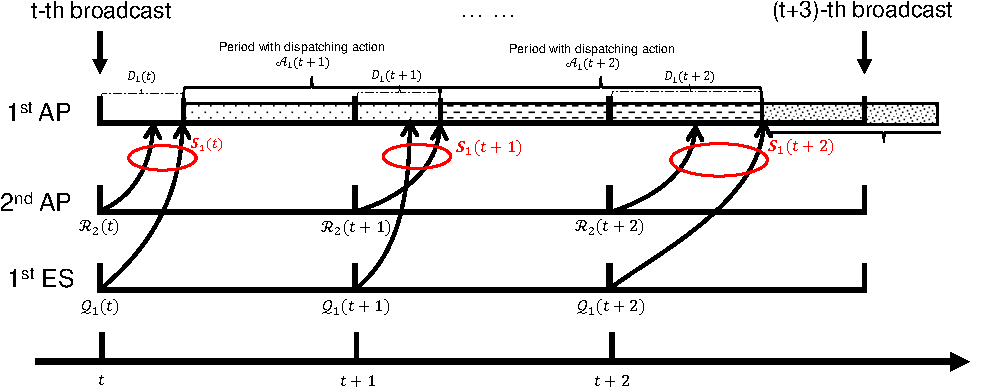
\includegraphics[width=0.60\textwidth]{brd-timeline.pdf}
    \caption{The timeline illustration of reception of OSI for the $1$-st AP where $2$-nd AP is in its \emph{conflict AP set} and $1$-st server is in its \emph{candidate server set}.}
    \label{fig:brd_timeline}
\end{figure*}

The $k$-th AP is able to collect its OSI $\Stat_{k}(t)$ at the $\mathcal{D}_{k}(t)$-th time slots of the $t$-th broadcast interval, where the \emph{\brlatency}~$\mathcal{D}_{k}(t)$ is a random variable.
It is assumed that $\mathcal{D}_{k}(t)$ follows identical and independent distribution in different broadcast interval.
% We refer to $\mathcal{D}_{k}(t)$ as the \brlatency~of the $k$-th AP at the $t$-th broadcast interval.
An example is given below to demonstrate how the \brlatency~affects the reception of OSI and the update of the dispatching strategy.

\begin{example}
    In Fig.\ref{fig:brd_timeline}, the $2$-nd AP and $1$-st server are in the \emph{conflict AP set} and \emph{candidate server set} of the $1$-st AP, respectively.
    At the beginning of the $t$-th broadcast interval, the dispatching actions $\mathcal{A}_{1}(t)$ is adopted by the $1$-st AP.
    After $\mathcal{D}_{1}(t)$ time slots, it updates the dispatching actions to $\mathcal{A}_{1}(t+1)$ based on its OSI $\Stat_{1}(t)$.
    In the $(t+1)$-th broadcast interval, the $1$-st AP will firstly keep the previous actions $\mathcal{A}_{1}(t+1)$, and then updates the actions $\mathcal{D}_{1}(t+1)$ time slots later based on $\Stat_{1}(t+1)$. The new action is denotes as $\mathcal{A}_{1}(t+2)$.
    The signaling latency $\mathcal{D}_1(t)$ and $\mathcal{D}_1(t+1)$ can be different.
\end{example}

\revision{
    \begin{remark}[Handling Broadcast Information Transmission Failure]
        % R1-1: How do you deal with the failed transmission of system state information?
        % R2-2: What if the information broadcast by the 2-nd AP is not received by the 1-st AP?
        The transmission failure of broadcast information could be easily handled with a simple retransmission schema.
        \hongyc{
            In one broadcast interval, if any AP could not receive the broadcast within a certain time limit which is denoted as $\tau_0$ (random variable with support $\set{0, \dots, \hat{\tau}_0}$), it will request a retransmission of the broadcast from the corresponding AP or edge server.
            The AP or edge server will immediately repeat the broadcast when receive the retransmission request, and we denote the Round-Trip Time (RTT) as $\tau_1$ (random variable with support $\set{0, \dots,\hat{\tau}_1}$).
            As the retransmission request or the repeated broadcast may fail again, we denote $\theta_\tau$ as the maximum retransmission times after which the transmission is believed to be received.
            The retransmission times until success is denoted as $\theta_\tau$.
            Therefore, the broadcast interval $T$ must be set to bound the maximum time elapsed $\hat{\theta}_{\tau}(\hat{\tau}_0+\hat{\tau}_1)$ to guarantee the complete reception of OSI in one broadcast interval.
            Moreover, $(\hat{\tau}_0+\hat{\tau}_1)$ is limited because of the original constraint of hops, and $\hat{\theta}_\tau$ is usually small.
            As a remark notice that the elapsed time $\theta_{\tau}(\tau_0+\tau_1)$ for the $k$-th AP at the $t$-th broadcast interval is exactly the \brlatency~$\Delay_k(t)$.
        }
    \end{remark}
}

The notations used throughout this paper are summarized as in Table \ref{table:symbols}.
\begin{table}[htp!]
    % \footnotesize
    \centering
    \caption{Table of notations and their descriptions throughout this paper.}
    \label{table:symbols}
    \begin{tabulary}{0.9\linewidth}{|p{1.8cm}|L|}
        \hline
        Notation                        & Description \\
        \hline
        $\mathcal{K}$                   & The denotation of AP set \\
        $\mathcal{M}$                   & The denotation of edge server set \\
        $\mathcal{K}_{m}$               & The potential AP set of the $m$-th edge server \\
        $\mathcal{M}_{k}$               & The candidate edge server set of the $k$-th AP \\
        $\ccSet_{k}$                    & The conflict AP set of the $k$-th AP  \\
        $\mathcal{J}$                   & The denotation of job types set \\
        $\lambda_{k,j}$                 & The average arrival job rate for the type-$j$ job on the $k$-th AP \\
        $c_{m,j}$                       & The average computation time for the type-$j$ job on the $m$-th edge server \\
        $L_{max}$                       & The maximum job number for each VM \\
        $t_B$                           & The duration of a broadcast interval \\
        $\Xi$                           & The maximum job uploading time \\
        $\xi$                           & The index of time slot of uploading time for one job \\
        $\mathbb{U}_{k,m,j}(\Xi)$       & The uploading latency distribution of the type-$j$ jobs from the $k$-th AP to the $m$-th edge server \\
        $\mathcal{R}_{k}(t)$            & The LSI of the $k$-th AP at the beginning of the $t$-th broadcast interval \\
        $\mathcal{Q}_{m}(t)$            & The LSI of the $m$-th edge server at the beginning of the $t$-th broadcast interval \\
        $D_{k}(t)$                      & The \brlatency~for the $k$-th AP at the $t$-th broadcast interval \\
        $\mathbb{D}(t)$                 & The vector of all \brlatency~ at the $t$-th broadcast interval \\
        $\Stat(t)$                      & The GSI at the $t$-th broadcast interval \\
        $\Stat_{k}(t)$                  & The OSI of the $k$-th AP at the $t$-th broadcast interval \\
        $\omega_{k,j}(t)$               & The dispatching action for type-$j$ job on the $k$-th AP at the beginning of $t$-th broadcast interval \\
        $\mathcal{A}_{k}(t)$               & The dispatching actions of the $k$-th AP at the beginning of $t$-th broadcast interval \\
        $\Policy(\Stat(t),\Delay(t))$   & The aggregation of individual policy all APs \\
        $\Baseline(\Stat(t),\Delay(t))$ & The proposed baseline policy \\
        $\gamma$                        & The discount factor \\
        $\beta$                         & The weight of overflow penalty \\
        $\mathcal{Y}_{n}$               & The $n$-th subset partition in which the APs update their dispatching actions parallelly \\
        $\tilde{\mathcal{A}}(t)$        & The aggregation of dispatching actions of the APs in the subset $\mathcal{Y}_{n}$, where $n \define t \pmod{N}$  \\
        $\hat{\mathcal{A}}(t)$          & The aggregation of dispatching actions of the APs not in the subset $\mathcal{Y}_{n}$, where $n \define t \pmod{N}$ \\
        \hline
    \end{tabulary}
\end{table}
    \section{POMDP-based Problem Formulation}
\label{sec:formulation}
%----------------------------------------------------------------------------------------%
In this section, we formulate the optimization of job dispatching problem of all APs as a Markov decision process (MDP).
Since each AP updates the job dispatching action according to OSI instead of GSI, the MDP problem is a partially observable MDP (POMDP).
Firstly, we give the definitions of \emph{dispatching policy} and \emph{cost function}, together with the \emph{system state} (i.e., the GSI) defined previously, to complete the MDP problem formulation.
% Specifically, the individual dispatching policy of one AP, the system dispatching policy, and the cost function are first defined below.

\begin{definition}[Dispatching Policy]
    The individual dispatching policy of the $k$-th AP, denoted as $\Omega_{k}$ ($\forall k \in\apSet$), maps from its OSI $\Stat_{k}$ and its \brlatency~$\mathcal{D}_{k}$ to the dispatching action for each job type, i.e.,
    \begin{align}
        \Omega_{k} \Paren{ \Stat_{k}(t), \mathcal{D}_{k}(t) }
        &\define \mathcal{A}_{k}(t+1)
        \nonumber\\
        &= \Brace{
            \omega_{k,j}(t+1) \Big| \forall j\in\jSpace
        }.
        \label{def:action}
    \end{align}

    The aggregation of individual policy of all APs is referred to as the system dispatching policy $\Policy$.
    Thus,
    {\small
    \begin{align}
        \Policy\Paren{ \Stat(t), \Delay(t) } \define \Brace{
            \Omega_{1}(\Stat_{1}(t), \mathcal{D}_{1}(t)), \dots, \Omega_{K}(\Stat_{K}(t),\mathcal{D}_{K}(t))
        },
    \end{align}
    }
    where $\Delay(t) \define \set{ \mathcal{D}_{1}(t), \dots, \mathcal{D}_{K}(t) }$.
\end{definition}

\revision{
    In this paper, the average job response time and packet drop rate are considered as the system cost.
    The job response time counts the number of broadcast intervals from job arrival to the accomplishment of computation, which includes the uploading time from the AP to the edge server, the waiting time in the processing queue and the job processing time on the edge server.
    According to the Little's law \cite{Little1961}, the average response time per job is proportional to the number of jobs in the system, given the job arrival rates at all the APs.
    % According to the Little's law \cite{Little1961}, the average response time per job, counting the number of broadcast intervals from job arrival to the accomplishment of computation, is proportional to the number of jobs in the system, given the job arrival rates at all the APs. %broadcast intervals
}%
Hence, we define the cost function per broadcast interval as follows, {given the information contained in periodic broadcast.}

\begin{definition}[Cost Function per Broadcast Interval]
    The cost function of the $t$-th broadcast interval with GSI $\Stat(t)$ is defined as
    {\small
    \begin{align}
        g\Paren{\Stat(t)} \define
            \sum_{m\in\esSet,j\in\jSpace}
            \Brace{&
                \sum_{k\in\apSet} \Inorm{\vec{R}^{(k)}_{m,j}(t,0)} + Q_{m,j}(t,0)
                \nonumber\\
                &~~~~~+ \beta \cdot I[Q_{m,j}(t,0)=L_{max}]
            },
    \end{align}
    }%
    where $\Inorm{\vec{x}}$ denotes the $L^1$-norm of the vector $\vec{x}$, $\sum_{k\in\apSet} \Inorm{\vec{R}^{(k)}_{m,j}(t,0)}$ measures the number of type-$j$ jobs being uploaded from the $k$-th AP to the $m$-th edge server, $Q_{m,j}(t,0)$ measures the number of type-$j$ jobs on the $m$-th edge server, and $\beta$ is the weight of overflow penalty.
    \deny{
        The cost function per broadcast interval could be taken as a uniform sampling of cost function per time slot.
    }
\end{definition}

Since the job dispatching in one broadcast interval will affect the GSI of the following broadcast intervals, we should consider the joint minimization of the costs of all the broadcast intervals.
Specifically, we consider the following discounted sum of the costs of all the broadcast intervals as the system objective.
{\small
\begin{align}
    &\bar{G}(\Stat(1), \Policy) \define
    \lim_{T \to \infty} \mathbb{E}^{\Policy}_{\set{\Stat(t)|\forall t}, \Delay}
    \Bracket{
        \sum_{t=1}^{T} \gamma^{t-1} g\Paren{\Stat(t)} \Big| \Stat(1)
    },
\end{align}
}%
where $\mathbb{E}^{\Policy}_{\set{\Stat(t)|\forall t}}[\cdot]$ denotes the expectation with respect to all possible system states in the future given scheduling policy $\Policy$, and $\gamma \in (0,1)$ is the discount factor.
Hence, the optimization of job dispatching policy can be formulated as the following minimization problem.
\begin{align}
    \textbf{P1:}~
    \min_{\Policy} \bar{G}(\Stat(1), \Policy).
\end{align}

If the GSI $\Stat(t)$ and \brlatency~$\Delay(t)$ are known to all the APs, the MDP in problem P1 can be solved via the following Bellman's equations as in \cite{sutton1998}.
\begin{align}
    &V\Paren{\Stat(t)} =g\Paren{\Stat(t)}
        + \gamma\mathbb{E}_{\Delay}\bigg\{
            \min_{\Policy(\Stat(t),\Delay(t))}
            \nonumber\\
            &\sum_{\Stat(t+1)} \Pr \Big\{ 
                \Stat(t+1) \Big| \Stat(t), \Policy(\Stat(t), \Delay(t)) \Big\} \cdot V\Big(\Stat(t+1)\Big)
            \bigg\},
    \label{eqn:sp_0}
\end{align}
where the value function $V(\Stat(t))$ of the optimal policy $\Policy^{*}$ (if GSI and \brlatency~are known to all the APs) is defined as follows.
\begin{align}
    &V\Paren{\Stat(t)} \define
    \lim_{T\to\infty} 
    \mathbb{E}^{\Policy^*}_{\set{\Stat(t)|\forall t}, \Delay} \Bracket{
        \sum_{t=1}^{T} \gamma^{t-1} g\Big( \Stat(t) \Big) \Big| \Stat(1)
    }.
    \label{eqn:val_f}
\end{align}
Moreover, the optimal dispatching policy $\Omega^{*}$ can be obtained by solving the right-hand-side (RHS) of the above Bellman's equations (\ref{eqn:sp_0}).

However, it is infeasible to solve the above Bellman's equations {and achieve the performance of $\Policy^*$ in our considered distributed dispatching scenario.}
This is because each AP (say the $k$-th AP) only has the knowledge of its own OSI $\Stat_{k}(t)$ and local \brlatency~$\mathcal{D}_{k}(t)$, but the optimal solution (dispatching actions of all APs) for the RHS of equation (\ref{eqn:sp_0}) depends on the GSI and the knowledge of global \brlatency.
Thus, problem P1 is actually a POMDP\revision{, which is further demonstrated by a toy example below.}
\revision{
    \begin{figure}[htp!]
        \centering
        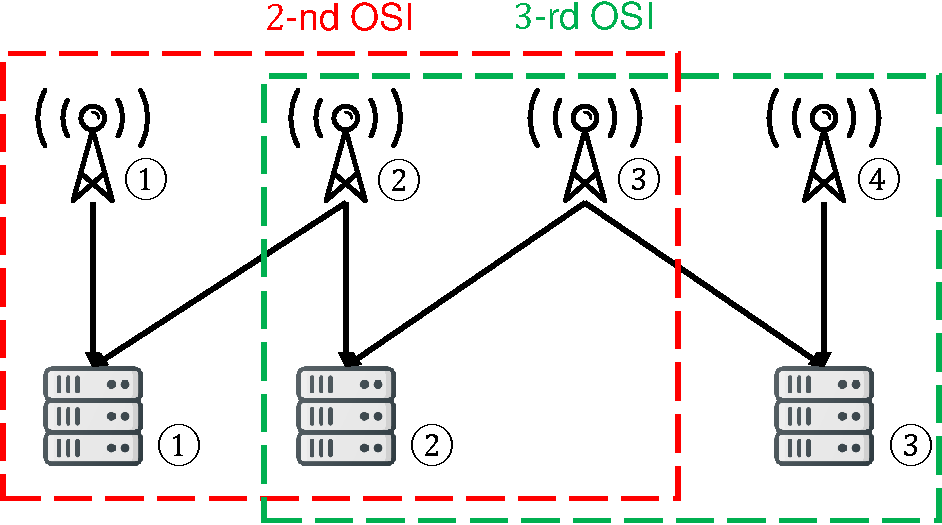
\includegraphics[width=0.45\textwidth]{images/osi-example.pdf}
        \caption{An example of system model, where the edge servers $1,2,3$ are collocated with the APs $1,2,4$, respectively.}
        \label{fig:osi_example}
    \end{figure}

    \begin{example}
        {%
            As illustrated in Fig.\ref{fig:osi_example}, there are four APs and three edge servers collocated with the APs, in the edge computing system, where the solid directed lines show all the possible job dispatching paths for the APs.
            For the $2$-nd AP, its OSI includes the state information of the APs indexed with $1,3$ and the edge servers indexed with $1,2$.
            The state information of the $3$-rd edge server is out of its scope.
            Moreover, the OSI of the $3$-rd AP (namely, the $3$-rd OSI) includes the state information of the APs indexed with $2,4$ and the edge servers indexed with $2,3$.
        }%
        Note that the prediction of future state distribution is essential for solving the RHS of equation (\ref{eqn:sp_0}).
        {%
            Without GSI, it is impossible to predict the future dispatching decisions of the $3$-rd AP from the perspective of the $2$-nd AP, since they observe different OSIs.
            It is thereby impossible for the $2$-nd AP to predict the future state distributions of the $2$-nd edge server, lack of the dispatching decisions of the $3$-rd AP.
            As a result, the evaluation of optimal value function of equation (\ref{eqn:val_f}) is infeasible at both $2$-nd and $3$-rd APs, and the distributed policy optimization for them is a POMDP.
        }
    \end{example}
}%

The general solution of POMDP is of huge complexity {as all the historical system states should be traced back in the current system state} \cite{IJCAI03-NairR,IJCAI99-BoutilierC}.
In this paper, we shall propose a novel low-complexity solution framework based on an analytical approximation of the value function $V(\cdot)$ and alternative actions update, where distributed job dispatching via the Bellman's equations becomes feasible
(the minimization at the RHS of equation (\ref{eqn:sp_0}) is solvable with the approximate value function)
even with OSI and local \brlatency.
%----------------------------------------------------------------------------------------%


    \section{Distributed Algorithm with Partial Information}
\label{sec:algorithm}

In this section, we shall introduce a novel approximation method to decouple the centralized optimization on the RHS of the Bellman's equations in equation (\ref{eqn:sp_0}) to each AP for arbitrary system state.
For the APs outside the conflict AP sets of each other, the update of dispatching actions at one AP will not affect the task computation originated from other APs.
Thus, the optimization of their dispatching actions can be decoupled.
On the other hand, for the APs within the same conflict AP set, the optimization of their dispatching actions is coupled.
Due to the unknown signaling latency, it is difficult for one AP (say the $k$-th AP) to predict the update of the dispatching actions at the other APs ($\forall k' \in\ccSet_{k}$).
Hence, cooperative optimization of dispatching actions for the APs within the same conflict AP set is infeasible.
\comments{In this section,} we introduce an alternative algorithm to optimize the dispatching actions of one AP in a conflict AP set in each broadcast interval periodically, while other APs maintain their dispatching actions in the previous broadcast interval.
Specifically, the proposed distributed algorithm consists of the following two steps:
%\hongyc{(move two steps adjacent in the following subsections)}
\begin{enumerate}
    \item We first introduce a baseline policy, use its value function to approximate the value function of the optimal policy $\Policy^*$, and derive the analytical expression of the approximate value function for arbitrary GSI in Section \ref{subsec:baseline}.
    \item With the approximate value function, an alternative action update algorithm, where only a subset of APs are selected to update their dispatching actions distributedly in each broadcast interval, is proposed in Section \ref{subsec:ap_alg}.
    Moreover, the analytical performance bound is also derived in Section \ref{subsec:analysis}.
\end{enumerate}
As a remark notice that solving the value function and then the RHS of the Bellman's equations are the two standard steps to solve an MDP problem with complete knowledge on system state.
In our proposed approximate solution framework, we extend this procedure to the POMDP problem in P1 by exploiting the structure of partially connected edge computing systems.
To the best knowledge of authors, a POMDP can hardly be solved via the Bellman's equations with full knowledge of system state in the existing literature.

\subsection{Baseline Policy and Approximate Value Function}
\label{subsec:baseline}
To alleviate the curse of dimensionality, we first use the baseline policy with fixed dispatching action to approximate value function at the RHS of the Bellman's equations in equation (\ref{eqn:val_f}).
Specifically, the baseline policy is elaborated below.

\begin{policy}[Baseline Policy]
    In the baseline policy $\Baseline$, each AP fixes the target processing edge server for each job type as the previous broadcast interval. Specifically, at the $t$-th broadcast interval,
    {\small
    \begin{align}
        \Baseline\Paren{\Stat(t),\Delay(t)} &\define \Bracket{ \Pi_{1}(\Paren{\Stat_{1}(t),\Delay(t)}, \dots, \Pi_{K}\Paren{\Stat_{K}(t),\Delay(t)} },
    \end{align}
    }
    where
    \begin{align}
        \Pi_{k}\Paren{\Stat_{K}(t),\Delay(t)}
        &= \Brace{
            \hat{\omega}_{k,j}(t+1) \Big| \forall j\in\jSpace
        }, \forall k\in\apSet.
    \end{align}
\end{policy}

Let $W_{\Baseline}(\cdot)$ be the value function of the baseline policy $\Baseline$, we shall approximate the value function of the optimal policy $V(\cdot)$ via $W_{\Baseline}$, i.e.,
{\small
\begin{align}
    &V\Paren{\Stat(t+1)} \approx W_{\Baseline}\Paren{\Stat(t+1)}
    \nonumber\\
    =& \sum_{m\in\esSet,j\in\jSpace}\Brace{
        \sum_{k\in\apSet} \tilde{W}^{\AP}_{k,m,j}(\Stat(t+1))
        +\tilde{W}^{\ES}_{m,j}(\Stat(t+1))
    },
    \label{eqn:baseline}
\end{align}
}
where $\tilde{W}^{\AP}_{k,m,j}(\Stat(t+1))$ denotes the cost raised by the type-$j$ jobs which are being transmitted from the $k$-th AP to the $m$-th edge server with the baseline policy $\Baseline$ and initial system state $\Stat(t+1)$, and $\tilde{W}^{\ES}_{m,j}(\Stat(t+1))$ denotes the cost raised by the type-$j$ jobs on the $m$-th server.
Their definitions are given below.
{\small
\begin{align}
    \tilde{W}^{\AP}_{k,m,j} \Paren{\Stat(t+1)} &\define
        \sum_{i=0}^{\infty} \gamma^{i+1} \mathbb{E}^{\Baseline}\Bracket{
            \Inorm{\vec{R}^{(k)}_{m,j}(t+i+1)}
        },
    \\    
    \tilde{W}^{\ES}_{m,j} \Paren{\Stat(t+1)} &\define
        \sum_{i=0}^{\infty} \gamma^{i+1} \mathbb{E}^{\Baseline}\Bracket{
            Q_{m,j}(t+i+1) +
            \nonumber\\
            &~~~~~~~~~~\beta I[Q_{m,j}(t+i+1) = L_{max}]
        }.
\end{align}
}

Moreover, the explicit expressions of $\tilde{W}^{\AP}_{k,m,j}(\Stat(t+1))$ and $\tilde{W}^{\ES}_{m,j}(\Stat(t+1))$ are derived in the following lemmas, respectively.

\begin{lemma}[Analytical Expression of $\tilde{W}^{\AP}_{k,m,j}$]
    \label{lemma:w_ap}
    \begin{align}
        &\tilde{W}^{\AP}_{k,m,j}\Paren{\Stat(t+1)} =
        \Inorm{
            \vecG{\Theta}^{(k, \Baseline)}_{m,j}(t+1) \times
            \Bracket{
                \mat{I} - \gamma \Gamma^{(k)}_{m,j}
            }^{-1}
        },
        \label{w_ap}
    \end{align}
    where $\mat{I}$ is the identity matrix, and $\vecG{\Theta}^{(k, \Baseline)}_{m,j}(t)$ and $\Gamma^{(k)}_{m,j}$ are defined below.
    \begin{itemize}
        \item {\small $\vecG{\Theta}^{(k,\Baseline)}_{m,j}(t) \define \Bracket{
            \theta^{(k,\Baseline)}_{m,j}(0,t),
            \theta^{(k,\Baseline)}_{m,j}(1,t),
            \dots,
            \theta^{(k,\Baseline)}_{m,j}(\Xi,t)
            }$},
        where 
        \begin{align}
            \theta^{(k)}_{m,j}(\xi,t) \define 
            \begin{cases}
                \lambda_{k,j} I[\omega_{k,j}(t)=m], & \xi=0
                \\
                \Pr\{R^{(k)}_{m,j}(\xi,t,0) = 1\}, & \text{otherwise}
            \end{cases}
        \end{align}
        \item $\Gamma^{(k)}_{m,j} \in \mathbb{R}^{(\Xi+1)\times(\Xi+1)}$ denotes the transition matrix whose entries are provided in Appendix \ref{append_1}.
    \end{itemize}
\end{lemma}
\begin{proof}
    Please refer to Appendix \ref{append_1}.
\end{proof}

\begin{lemma}[Analytical Expression of $\tilde{W}^{\ES}_{m,j}$]
    \label{lemma:w_es}
    {\small
    \begin{align}
        &\tilde{W}^{\ES}_{m,j}\Paren{\Stat(t+1)}
    = \sum_{i=0,\dots,\frac{\Xi}{T}} \gamma^{i} \mathbb{E}^{\Baseline}[ Q_{m,j}({t+i+1}) | \Stat(t+i)]
    \nonumber\\
    &~~~~~~~~~~~~+ \gamma^{\frac{\Xi}{T}} 
    \vecG{\nu}({t+\frac{\Xi}{T}+1})
    \Paren{
        \mat{I} - \gamma \mat{P}^{\Baseline}_{m,j}(t)
    }^{-1} \vec{g}',
        \label{w_es}
    \end{align}   
    }
    where $\vecG{\nu}_{m,j}(t)$, $\mat{P}_{m,j}(\beta_{m,j}(t))$, $\beta_{m,j}(t)$ and $\vec{g}$ are defined below.
    \begin{itemize}
        \item {\small
        $\vecG{\nu}_{m,j}(t) \define [\Pr\{Q_{m,j}(t)=0\}, \dots, \Pr\{Q_{m,j}(t)=L_{max}\}]$
        }.
        \item $\vec{g} \in \mathbb{R}^{(L_{max}+1) \times 1}$, and its $i$-th entry is
        \begin{align}
            [\vec{g}]_{i} \define 
            \begin{cases}
                i, & i=0,1,\dots,L_{max}-1
                \\
                L_{max}+\beta, & \text{otherwise}
            \end{cases}.
            \label{eqn:g_vec}
        \end{align}
        \item The expression of $\mathbb{E}^{\Baseline}[ Q_{m,j}({t+i+1}) | \Stat(t+i)]$ is elaborated in Appendix \ref{append_2}.
        \item $\mat{P}^{\Baseline}_{m,j}(t) \in \mathbb{R}^{(L_{max}+1) \times (L_{max}+1)}$ denotes the transition matrix under baseline policy $\Baseline$ whose entries are described in Appendix \ref{append_2}.
    \end{itemize}   
\end{lemma}
\begin{proof}
    Please refer to Appendix \ref{append_2}.
\end{proof}

\subsection{Distributed Action Update}
\label{subsec:ap_alg}
Although the optimal value function has been approximated via the baseline policy in the previous part, it is still infeasible for all the APs to solve the RHS of the Bellman's equations in a distributed manner with OSI and local \brlatency~only.
This is because the evaluation of equation (\ref{w_ap}) and (\ref{w_es}) requires the knowledge of GSI and \brlatency~at all APs.
Instead, it is feasible for part of APs to update their dispatching actions distributed and achieve a better performance compared with baseline policy.
Hence, we first define the following sequence of AP subsets, where each subset are selected to update dispatching actions periodically.
\begin{definition}[Subsets Partition]
    Let $\mathcal{Y}_{1}, \dots, \mathcal{Y}_{N} \subseteq \ccSet$ be a collection of subsets of AP set $\apSet$, which satisfy
    \begin{align}
        &\bigcup_{n=0,\dots,N-1} \mathcal{Y}_{n} = \apSet
        \label{eqn:subset_cup}
        \\
        \esSet_{y} \cap \esSet_{y'} &=\emptyset, y' \neq y~(\forall y',y \in \mathcal{Y}_{n}).
        \label{eqn:subset_disjoint}
    \end{align}
\end{definition}
The condition in equation (\ref{eqn:subset_cup}) is to ensure all the APs can update their dispatching actions periodically; whereas the condition in equation (\ref{eqn:subset_disjoint}) is to ensure APs in the conflict AP sets of each other will not update their dispatching actions in the same broadcast interval.
For example, as illustrated in Fig.\ref{fig:system}, the AP set $\apSet$ could be decomposed of two subsets as $\set{1,3}$ and $\set{2}$.
The subset partition is not trivial and {a partition minimizing the update period $N$ is preferred}.
A heuristic greedy algorithm is given as follows in Algorithm \ref{alg_0}.
\begin{algorithm}[ht]
    \caption{Greedy Subset Partition Algorithm}\label{alg_0}
    \DontPrintSemicolon % Some LaTeX compilers require you to use \dontprintsemicolon instead
    \KwIn{$\apSet, \set{\esSet_{k}, \forall k\in\apSet}$ }
    \KwOut{a subset partition $\set{ \mathcal{Y}_{n} }$}
    Initialize a subset partition as $\mathcal{Y}_{n} = \set{n}$ ($\forall n\in\apSet$).\;
    \While{ $\exists \mathcal{Y}_a$ and $\mathcal{Y}_b$ ($a \neq b$), $\cup\set{ \esSet_{y}|y\in\mathcal{Y}_a } \bigcap \cup\set{ \esSet_{y}|y\in\mathcal{Y}_b } \neq \emptyset$ }
    {
        Count number of subsets in the current subset partition which have disjoint candidate set with $\mathcal{Y}_n$ ($\forall n$), denoted the number as $I_{n}$.\;
        $\tilde{n} \gets \arg\min_{n} I_{n}$\;
        Merge the subset $Y_{\tilde{n}}$ with one of its disjoint subsets.\;
    }
\end{algorithm}

At the $t$-th broadcast interval, the APs in the subset indexed with $n \define t \pmod{N}$ update their dispatching actions, while the other APs keep the same dispatching actions as the previous broadcast interval.
Hence, let
\begin{align}
    \tilde{\mathcal{A}}(t) \define \Brace{ \tilde{\omega}_{y,j}(t) \Big| \forall y\in\mathcal{Y}_{n},j\in\jSpace }
\end{align}
be the aggregation of dispatching actions the APs in the subset $\mathcal{Y}_{n}$, and
\begin{align}
    \hat{\mathcal{A}}(t) \define \Brace{ \hat{\omega}_{y,j}(t) \Big| \forall y\notin\mathcal{Y}_{n}, j\in\jSpace}
\end{align}
be the aggregation of dispatching actions of the rest APs, which are the same as the previous broadcast interval.
At the $t$-th broadcast interval, the optimization of $\tilde{\mathcal{A}}(t)$ at the RHS of the Bellman's equations can be rewritten as the following problem.
{\small
\begin{align}
    \textbf{P2:}~
    \min_{ \tilde{\mathcal{A}}(t) }
    &\sum_{\Stat(t+1)} \Pr\Brace{
        \Stat(t+1) \Big| \Stat(t), \tilde{\mathcal{A}}(t), \hat{\mathcal{A}}(t)
    } \cdot W_{\Baseline}\Paren{\Stat(t+1)}.
\end{align}
}

Moreover, we have the following conclusion on the decomposition of P2.
\begin{lemma}[]
    The optimization problem in P2 can be equivalently decoupled into local optimization problems at APs \comments{for each subset partition}.
    Specifically, \comments{the local optimization for the APs in the $n$-th subset ($\forall n$) can be written as}
    \small{\begin{align}
        &\textbf{P3:}~
        \min_{ \tilde{\mathcal{A}}(t) } \sum_{y\in\mathcal{Y}_{n}}
        \mathbb{E}_{\set{ \Stat_{y}(t+1)|\Stat_{y}(t), {\mathcal{A}}_{y}(t) }}
        \nonumber\\
        &~~~~\sum_{ j\in\jSpace,m\in\esSet_{y} } \Brace{
            \tilde{W}^{\AP}_{k,j}\Paren{\Stat_{y}(t+1)}
            +\tilde{W}^{\ES}_{m,j}\Paren{\Stat_{y}(t+1)}
        }.
        \label{eqn:partial}
    \end{align} }
    \label{lemma:w_partial}
\end{lemma}
\begin{proof}
    At the $t$-th broadcast interval, the $y$-th AP in the subset $\mathcal{Y}_{n}$ updates its dispatching actions, which could only affect the future cost raised on itself and its corresponding \emph{candidate server set}, i.e., the part of its OSI.
    Hence, it's obvious that the expression of equation (\ref{w_ap}) and equation (\ref{w_es}) on the RHS of the Bellman's equations could be reduced into the form based only on the OSI of the $y$-th AP ($\forall y\in\mathcal{Y}_{n}$), \comments{and linearly summed as illustrated in equation (\ref{eqn:partial})}.
\end{proof}

The optimization of \comments{collection of dispatching actions $\set{\hat{\omega}_{y,j}|\forall j\in\jSpace}$} for the $y$-th AP ($\forall y\in\mathcal{Y}_{n}$) in P3 could be achieved via searching all the edge servers in $\esSet_{y}$, \comments{whose computational complexity is $O(J|\mathcal{M}_{y}|)$}.
As a result, the overall algorithm of job dispatching is elaborated in Algorithm \ref{alg_1}.
\begin{algorithm}[ht]
    \caption{\comments{Online Alternative Actions Update Algorithm}}\label{alg_1}
    \DontPrintSemicolon % Some LaTeX compilers require you to use \dontprintsemicolon instead
    % \KwIn{$\Stat(t), \Delay(t)$}
    % \KwOut{$\tilde{\mathcal{A}}(t)$}
    Initialize all the APs with heuristic dispatching actions $\set{\hat{\omega}_{k,j}(0)|\forall k\in\apSet,j\in\jSpace}$.\;
    \For{$t=0,1,2,\dots$}{
        \tcc{Get the index of the subset to update at $t$.}
        $n \gets t \pmod{N}$\;
        \tcc{Parallelly update the actions of APs in the subset $\mathcal{Y}_{n}$.}
        \ForPar{$y \in \mathcal{Y}_{n}$}{
            \tcc{Each AP observes its LSI asynchronously.}
            The $y$-th AP observes $\Stat_{y}(t)$ after $\mathcal{D}_{y}(t)$.\;
            \tcc{Then update actions by solving P3.}
            solving P3 with $\Stat_{y}(t), \mathcal{D}_{y}(t)$ and obtain $\set{\tilde{\omega}_{y,j}(t+1)|\forall j\in\jSpace}$\;
        }
        $\tilde{\mathcal{A}}(t+1) \gets \set{\tilde{\omega}_{y,j}(t+1)|\forall y\in\mathcal{Y}_{n},j\in\jSpace}$\;
        \tcc{The other APs fix the actions as the previous interval.}
        $\hat{\mathcal{A}}(t+1) \gets \hphantom{~~} \set{ \tilde{\omega}_{y,j}(t) | \forall y\in\mathcal{Y}_{n-1},j\in\jSpace }$\;
        $\hphantom{~~~~~~~~~~~~~~~~~} \cup \set{ \hat{\omega}_{y,j}(t) | \forall y\notin\mathcal{Y}_{n-1},j\in\jSpace }$\;
    }
\end{algorithm}

Moreover, we use the following example to illustrate the procedure of Algorithm \ref{alg_1}.
\begin{example}
    \label{exp:update}
    \comments{
       In Fig.\ref{fig:system}, the AP set $\apSet$ could be partitioned into two subsets which are denoted as $\mathcal{Y}_{0} = \set{1,3}$ and $\mathcal{Y}_{1} = \set{2}$, respectively.
       As illustrated in Fig.\ref{fig:update_timeline}, in the $1$-st interval the APs in subset $\mathcal{Y}_{0}$ would update their dispatching actions by solving P3 which consists of $\tilde{\mathcal{A}}(1)$, while the AP in subset $\mathcal{Y}_{1}$ fix its actions which consists of $\hat{\mathcal{A}}(1)$.
       Then in the $2$-nd interval, the APs in subset $\mathcal{Y}_{0}$ in turn fix their actions $\tilde{\mathcal{A}}(1)$ which consists of $\hat{\mathcal{A}}(2)$, while 
       the AP in subset $\mathcal{Y}_{1}$ updates the dispatching actions based on $\hat{\mathcal{A}}(1)$ which consists of $\tilde{\mathcal{A}}(2)$.
       This procedure repeats with the period $N=2$.
    }
    \begin{figure*}[htp!]
        \centering
        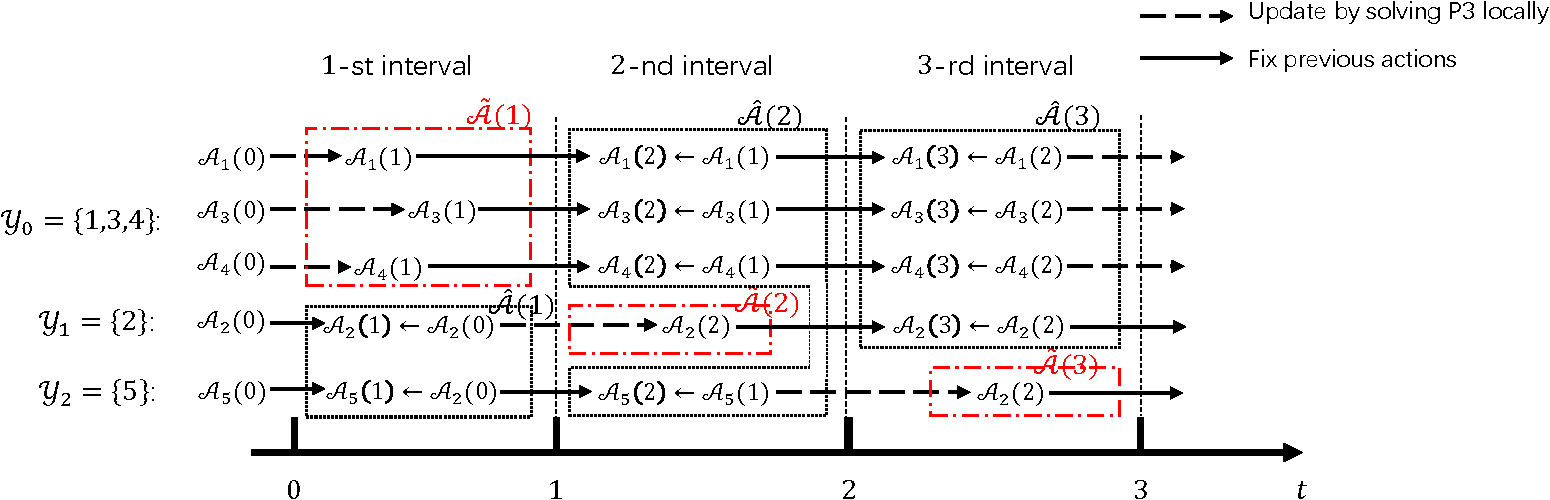
\includegraphics[width=0.60\textwidth]{update-timeline.pdf}
        \caption{The Illustration of Example \ref{exp:update}.}
        \label{fig:update_timeline}
    \end{figure*}
\end{example}

As a remark notice that Algorithm \ref{alg_1} leads to a time-variant policy, which is referred as the proposed policy $\tilde{\Policy}$.
At the $t$-th broadcast interval, the dispatching actions is given by
\begin{align}
    \tilde{\Policy}(\Stat(t), \Delay(t)) \define \tilde{\mathcal{A}}(t+1) \cup \hat{\mathcal{A}}(t+1).
\end{align}

Moreover since in Algorithm \ref{alg_1}, the computation complexity at each AP scales linearly with respect to \comments{the size of candidate edge server set}, it can be deployed in a scenario with massive APs and edge servers, as long as the \comments{the available number of edge servers for each AP} is limited.

\subsection{Analytical Performance Bound}
\label{subsec:analysis}
In most of the existing approximate MDP solutions\comments{(need ref)}, the performance is difficult to bound analytically as the approximate value function has no accurate meaning on the system cost or utility.
In the proposed algorithm, however, we derive the analytical expression for the baseline policy as the approximate.
Hence, the alternative dispatching action update can ensure to achieve a better performance than the baseline policy.
This conclusion is summarized below.
% We have the following conclusion on the performance of the above proposed algorithm.
\begin{lemma}[Analytical Cost Upper Bound]
    \label{lemma:bound}
    Let $W_{\tilde{\Policy}}(\cdot)$ be the value function (average cost) of the proposed policy $\tilde{\Omega}$, i.e.,
    \begin{align}
        W_{\tilde{\Policy}}(\Stat) \define
        \sum_{t'=1}^{\infty} \gamma^{t'-1} \mathbb{E}^{ \tilde{\Policy} } \Bracket{
            g\Paren{\Stat(t'), \tilde{\Policy}(\Stat(t'),t')} \Big| \Stat(1)=\Stat
        },
    \end{align}
    we have
    \begin{align}
        V(\Stat)
        \leq W_{\tilde{\Policy}}(\Stat)
        \leq W_{\Baseline}(\Stat),
        \forall \Stat.
    \end{align}
\end{lemma}
\begin{proof}
    Please refer to Appendix \ref{append_3}.
\end{proof}
Therefore, $W_{\Baseline}(\Stat)$ derived in equation (\ref{eqn:baseline}) can be used as the analytical cost upper bound of the proposed policy $\Baseline$.
Moreover, Lemma \ref{lemma:bound} also implies that the proposed policy with fixed service edge server for each AP, as long as the {static dispatching policy} is used as the baseline policy.
% the average system cost of the proposed algorithm is upper bounded by $W_{\Baseline}(\Stat)$ ($\forall \Stat$) which means it is always better than the baseline policy. 

% \subsection{Scalability Analysis}
% \hongyc{(append the subsection to show that scalability is good, when connection is uniform with APs and edge servers.)}
%----------------------------------------------------------------------------------------%
%----------------------------------------------------------------------------------------%
    \section{Performance Evaluation}
\label{sec:evaluation}
In this section, we evaluate the performance of the proposed low-complexity dispatching policy $\tilde{\Policy}$ by numerical simulations.
The experiment setup and performance benchmarks are elaborated in Section \ref{subsec:setup}.
The simulation results are illustrated in Section \ref{subsec:basic}.
The sensitivity study on parameters is also applied to provide some insights on the robustness of the proposed policy in Section \ref{subsec:advance}.

\subsection{Experiment Setup}
\label{subsec:setup}
In the simulation, we assume that there are $K=15$ APs, $M=10$ processing servers and $J=10$ types of jobs in the system.
One broadcast interval is consist of $t_{B}=25$ time slots.
% The time slot duration is $20$ milliseconds and one broadcast interval consists of $t_{B}=25$ time slots.
The network topology among APs is generated according to Barab\'asi-Albert (BA) model \cite{albert1999diameter} and the APs and processing servers are randomly placed.
% Under this network topology setup with degree as $3$, the subset partition algorithm \ref{alg_0} could reduce the update period $N$ from $15$ to $6$ time slots.
% The BA model is parameterized by $n$ and $m$ and produces a graph with $n$ vertices and $m$ edges such that the degree distribution follows a power-law.
The arrival traces and job processing time for each job type are extracted from Google cluster traces \cite{clusterdata:Reiss2011} and then randomly assigned on APs and edge servers, respectively.
The maximum uploading latency is $\Xi = 3t_B$, and the distribution of $\mathbb{U}_{k,m,j}(\Xi)$ ($\forall k\in\apSet, m\in\esSet_{k}, j\in\jSpace$) is arbitrarily generated within the support $\set{0, 1, \dots, \Xi}$.
The \brlatency~ is with an integer support from $0.7t_B$ to $0.9t_B$ time slots.
Each queue for VMs on edge server is with maximum queue length $L_{max}=50$, i.e., there would be at most $50$ jobs on one edge server.
The discount factor $\gamma$ is $0.95$ and the overflow penalty weight $\beta$ is $120$.

\delete{TMC-v1}{
    In the simulation, we assume that there are $K=15$ APs, $M=10$ edge servers and $J=10$ types of jobs in the system.
    One broadcast interval is consist of $t_B=25$ time slots. The network topology among APs is generated according to 
    The time slot duration is $20$ milliseconds and one broadcast interval consists of $t_{B}=25$ time slots, i.e., its duration is $1$ second.
    Each AP would have at most $3$ edge servers in its candidate set, and the adjacency matrix for generated bipartite map between APs and edge servers is illustrated in Fig.\ref{fig:bipartite}.

    % arbitrarily generated with: summed average arrival \emph{smaller than} summed departure rate, for each job type.
    {
        The other parameters for signaling, job processing and uploading are generated arbitrarily following no presumed distributions.
        Specifically, the job processing related parameters are chosen to satisfy the system stability, i.e., the average arrival rate is always smaller than the departure rate on one edge server for each job type.
    }
    The \brlatency~is a discrete random variable with an integer support from $12$ to $20$ time slots.
    The maximum uploading latency is $3$ seconds, i.e., $\Xi = 3t_B$, and the distribution of $\mathbb{U}_{k,m,j}(\Xi)$ ($\forall k\in\apSet, m\in\esSet_{k}, j\in\jSpace$) is arbitrarily generated within the support $\set{0, 1, \dots, \Xi}$.
    The expected computation time $c_{m,j}$ ($\forall m\in\esSet, j\in\jSpace$) is an integer uniformly generated in the range $[50,125]$ (with the unit of time slot) in each figure.
    Each queue for VMs on edge server is with maximum queue length $L_{max}=50$, i.e., there would be at most $50$ jobs on one edge server.
    The arrival rate in each time slot is uniformly generated from the range $[0.02, 0.03]$ for each job type at each AP in each figure.
    The discount factor $\gamma$ is $0.95$ and the penalty weight $\beta$ is $30$.
    % The arrival rate is taken as small probability with enough APs in the system, and correspondingly enough edge servers for the processing.
}

%-----------------------------------------------------------------------%
\begin{figure}[ht]                                                      %
    \centering                                                          %
    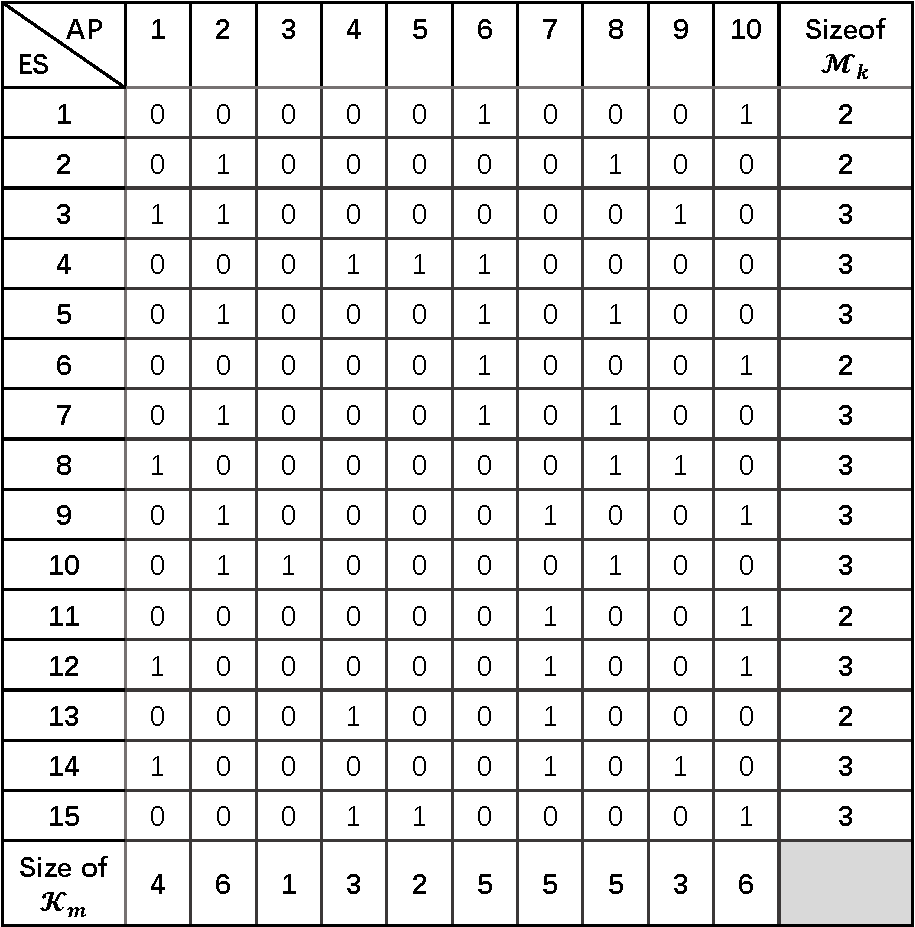
\includegraphics[width=0.45\textwidth]{sim-bipartite.pdf}           %
    \caption{The illustration of adjacency matrix between APs and edge servers in the simulation.}
    \label{fig:bipartite}                                               %
\end{figure}                                                            %
%-----------------------------------------------------------------------%

%-----------------------------------------------------------------------%
\begin{figure}[ht]                                                      %
    \centering                                                          %
    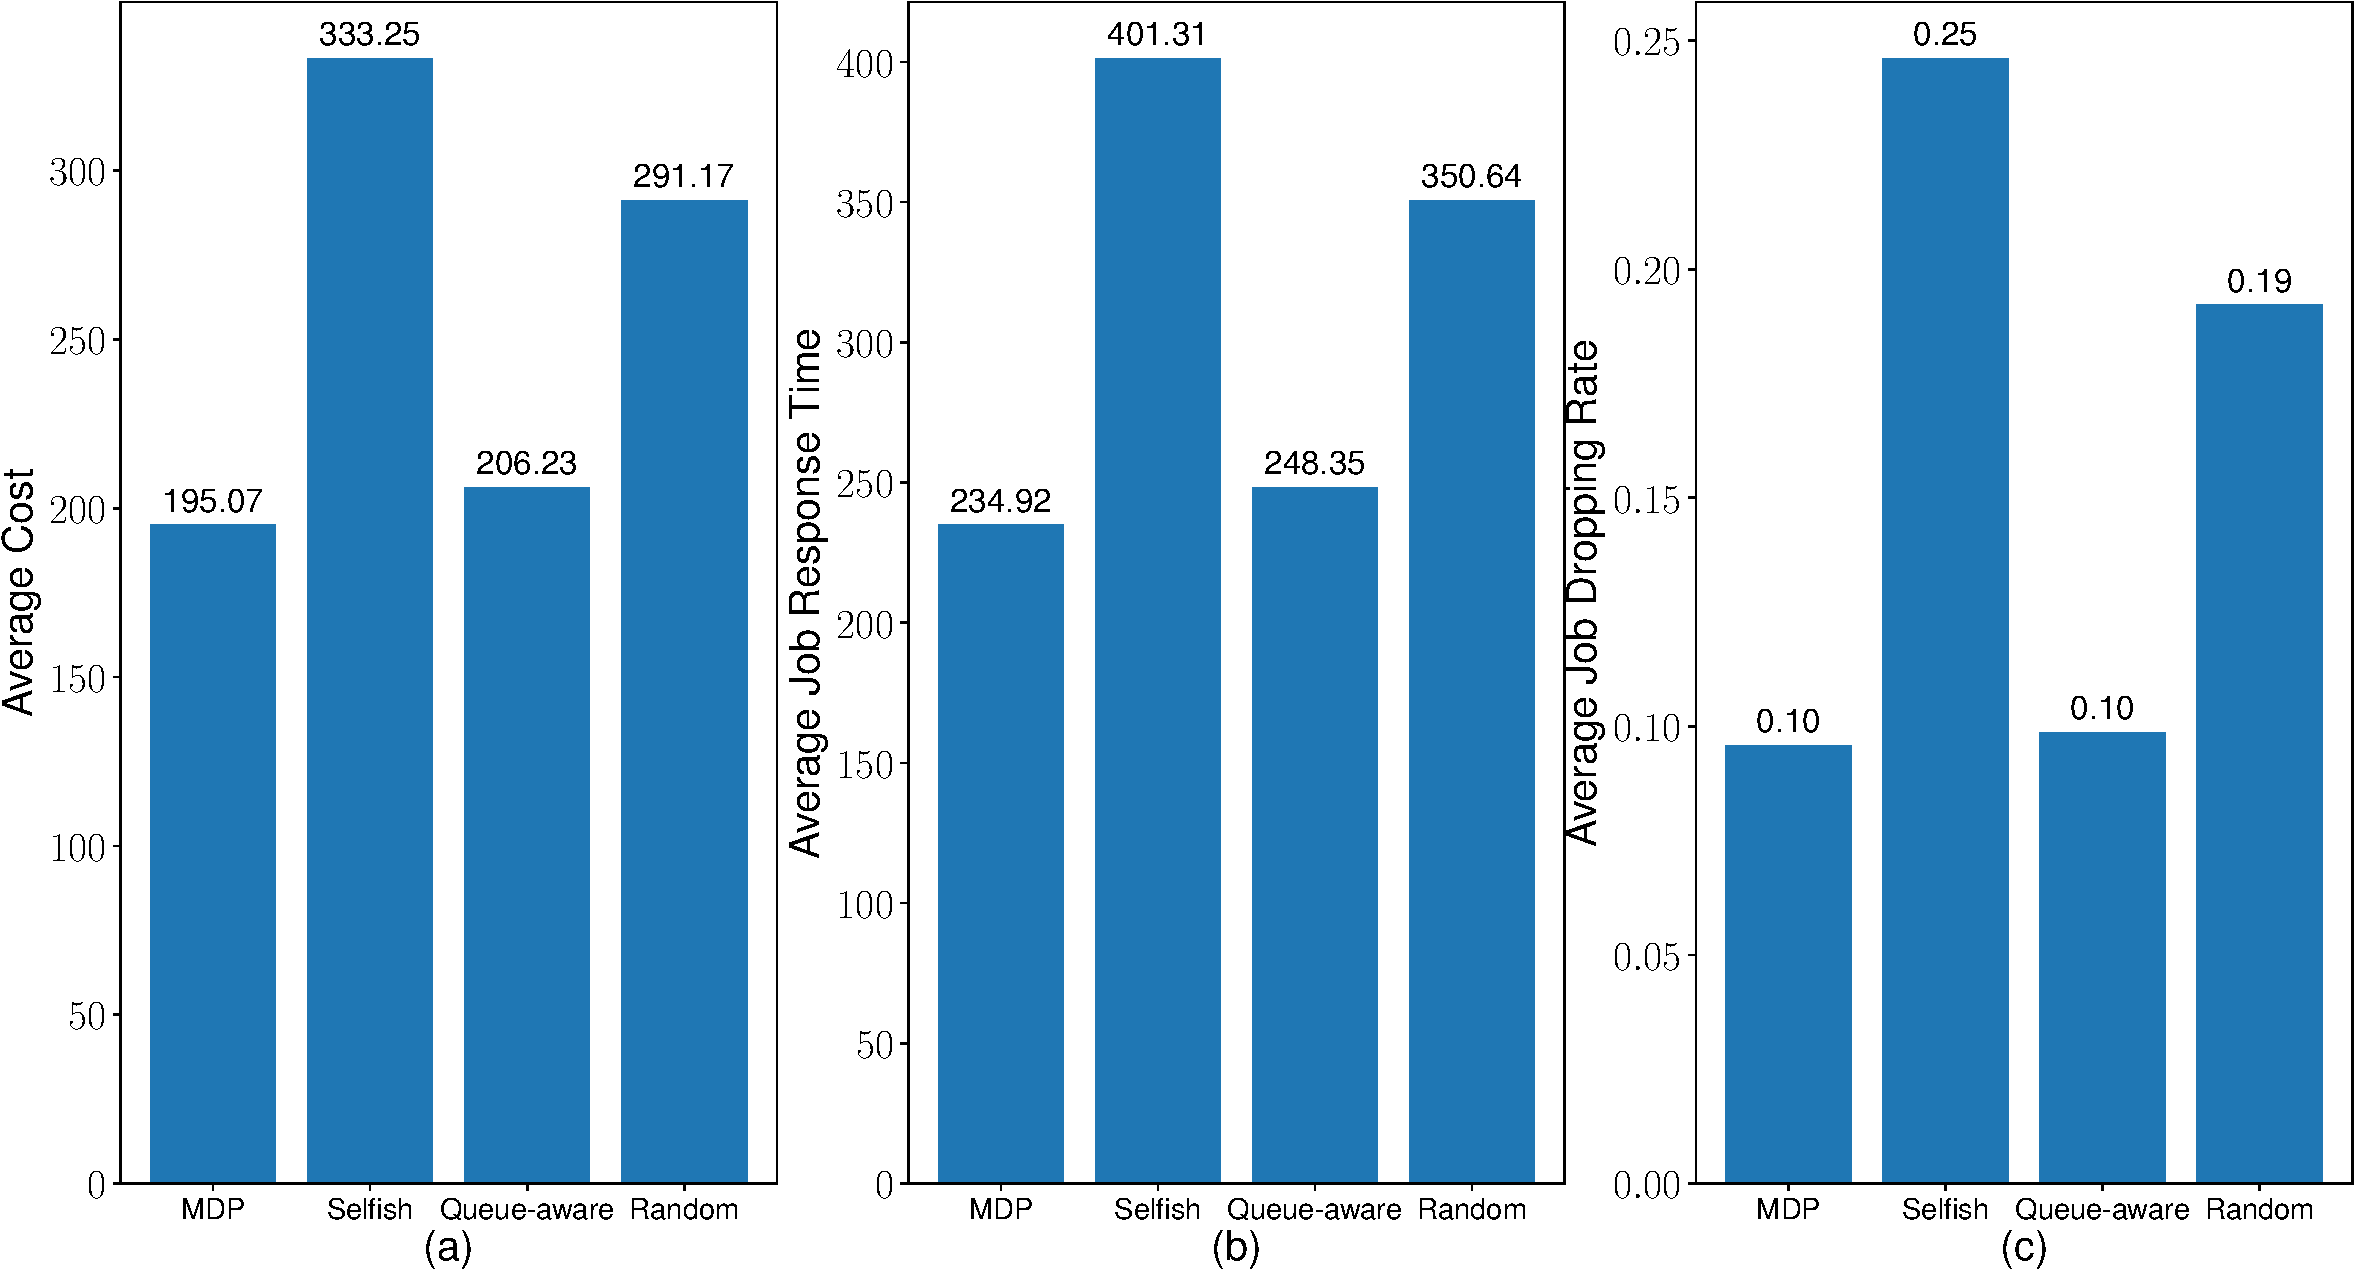
\includegraphics[width=0.45\textwidth]{the-bar-graph.pdf}               %
    \caption{Illustration of performance metrics comparison with benchmarks.}
    \label{fig:bar_plot}                                                %
\end{figure}                                                            %
%-----------------------------------------------------------------------%

%NOTE: Benchmark Elaboration
We also propose {three heuristic benchmarks to profile the performance of the proposed \algname}, which are listed as follows.
\begin{itemize}
    \item \textbf{Random Dispatching Policy}:
            Randomly choose a dispatching edge server in each time slot; 
    \item \textbf{Selfish Policy}:
            Always choose the edge server with the minimum sum of the expected uploading time and processing time;
    \item \textbf{Queue-aware Policy}:
            Always choose the edge server with the minimum sum of expected uploading time, processing time and queueing time based on the observation of outdated queue states.
\end{itemize}
Moreover, we choose the Selfish Policy as the initial dispatching action for our proposed algorithm (Algorithm \ref{alg_1}).

%NOTE: Basic Performance
\subsection{Performance Analysis}
\label{subsec:basic}
As illustrated in Fig.\ref{fig:bar_plot}(a), the proposed algorithm (MDP Policy) outperforms all the benchmarks in the average system cost.
% Moreover, the Queue-aware Policy has better performance than the other benchmarks due to its capability of adapting dispatching action according to the outdated observation of queueing state.
More insights on the performance comparison are provided in Fig.\ref{fig:bar_plot}(b) and (c).
In the former figure, the average job response times, measuring the average number of broadcast intervals from job's arrival at one AP to the completeness of computation at one edge server, are compared.
It can be observed that the proposed policy still outperforms all the benchmarks.
In Fig.\ref{fig:bar_plot}(c), the job dropping rates, measuring the ratio of jobs dropped by edge servers due to queue overflow, are also compared.
It is shown that the proposed policy outperforms other three benchmarks with the minimum average cost and job response time.
\hongyc{And there is no dropping jobs incurred compared with the Selfish policy, which is the initial baseline policy for our proposed algorithm.}
Finally, an realization of job dispatching is illustrated in Fig.\ref{fig:general_timeline}, where the number of jobs in the system is plot versus the index of broadcast interval.
It can be observed that the proposed policy manage to keep the number of jobs in lower level, compared with the other benchmarks.
This demonstrates its high dispatching efficiency.

\hongyc{
    In Fig. \ref{fig:semi-bound}, it shows that the performance of proposed policy is always below the semi-analytical cost upper bound $W^{(T)}_{\hat{\Baseline}}(\Stat)$ (with a typical initial state with no jobs in the system) for any $T$ , and the performance gap $e(T)$ decreases monotonically with respect to $T$.
}%

%-----------------------------------------------------------------------------------------------%
\begin{figure}[ht!]                                                                             %
    \centering                                                                                  %
    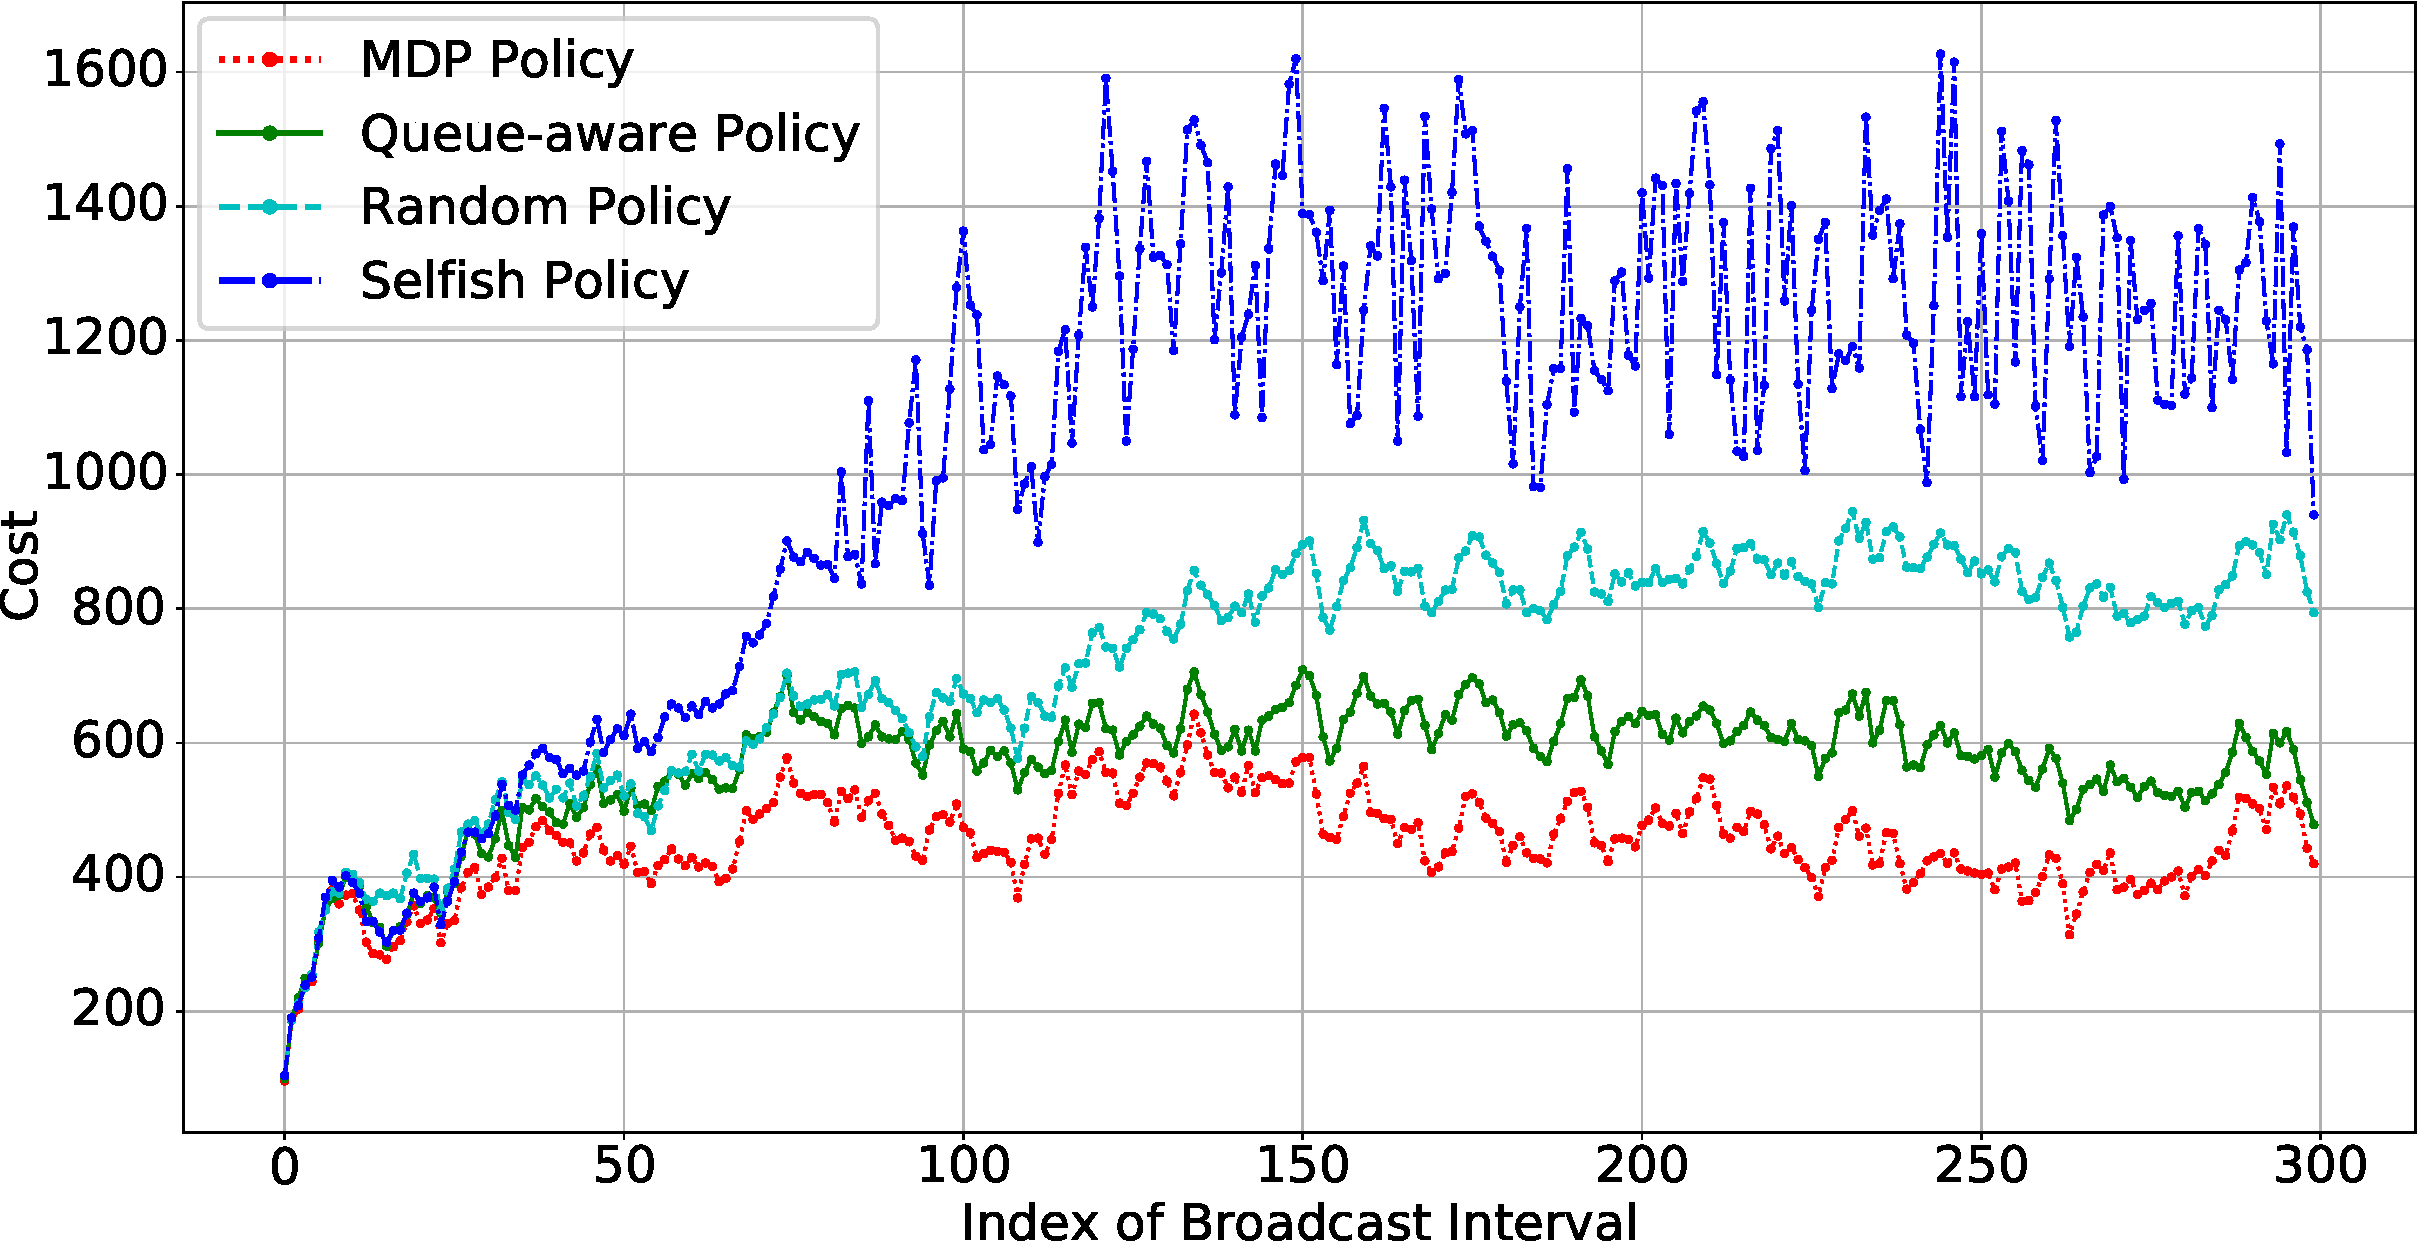
\includegraphics[width=0.45\textwidth]{the-cost-timeline-alt.pdf}                     %
    \caption{Illustration of cost versus index of broadcast interval.}
    \label{fig:general_timeline}                                                                %
\end{figure}                                                                                    %
%-----------------------------------------------------------------------------------------------%

%TODO:
%-----------------------------------------------------------------------------------------------%
\begin{figure}[ht!]                                                                             %
    \centering                                                                                  %
    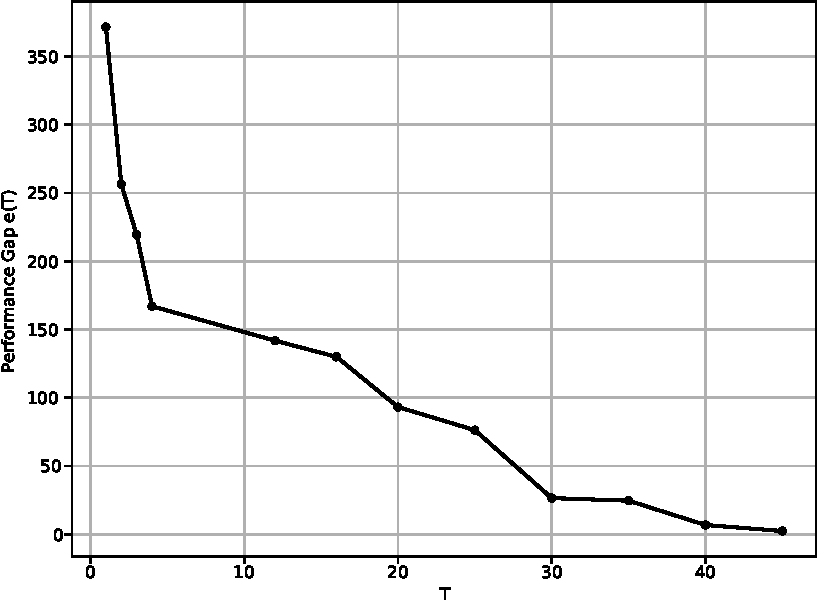
\includegraphics[width=0.45\textwidth]{the-semi-bound-analysis.pdf}                     %
    \caption{Illustration of Performance Gap Monotonically Decreasing.}
    \label{fig:semi-bound}                                                                %
\end{figure}                                                                                    %
%-----------------------------------------------------------------------------------------------%

%NOTE: Reinforcement Learning Analysis
\subsection{Convergence Analysis}
\label{subsec:converge}
The convergence property of the proposed reinforcement learning algorithm is illustrated in Fig.\ref{fig:rl_plot}.
It can be observed that the learning procedures for all the three statistical parameters converge after $90$ broadcast intervals, which is far before the system achieving the balance dynamic under the dispatching policy.
On the other hand, the number of observations required for the convergence of conventional reinforcement learning algorithms is usually larger for enormous system and action space.
This demonstrates the efficiency of the proposed reinforcement learning algorithm, which benefits from the derived expression the the approximate value function.
% performance compared with prior-knowledge
\begin{figure}[ht!]
    \centering
    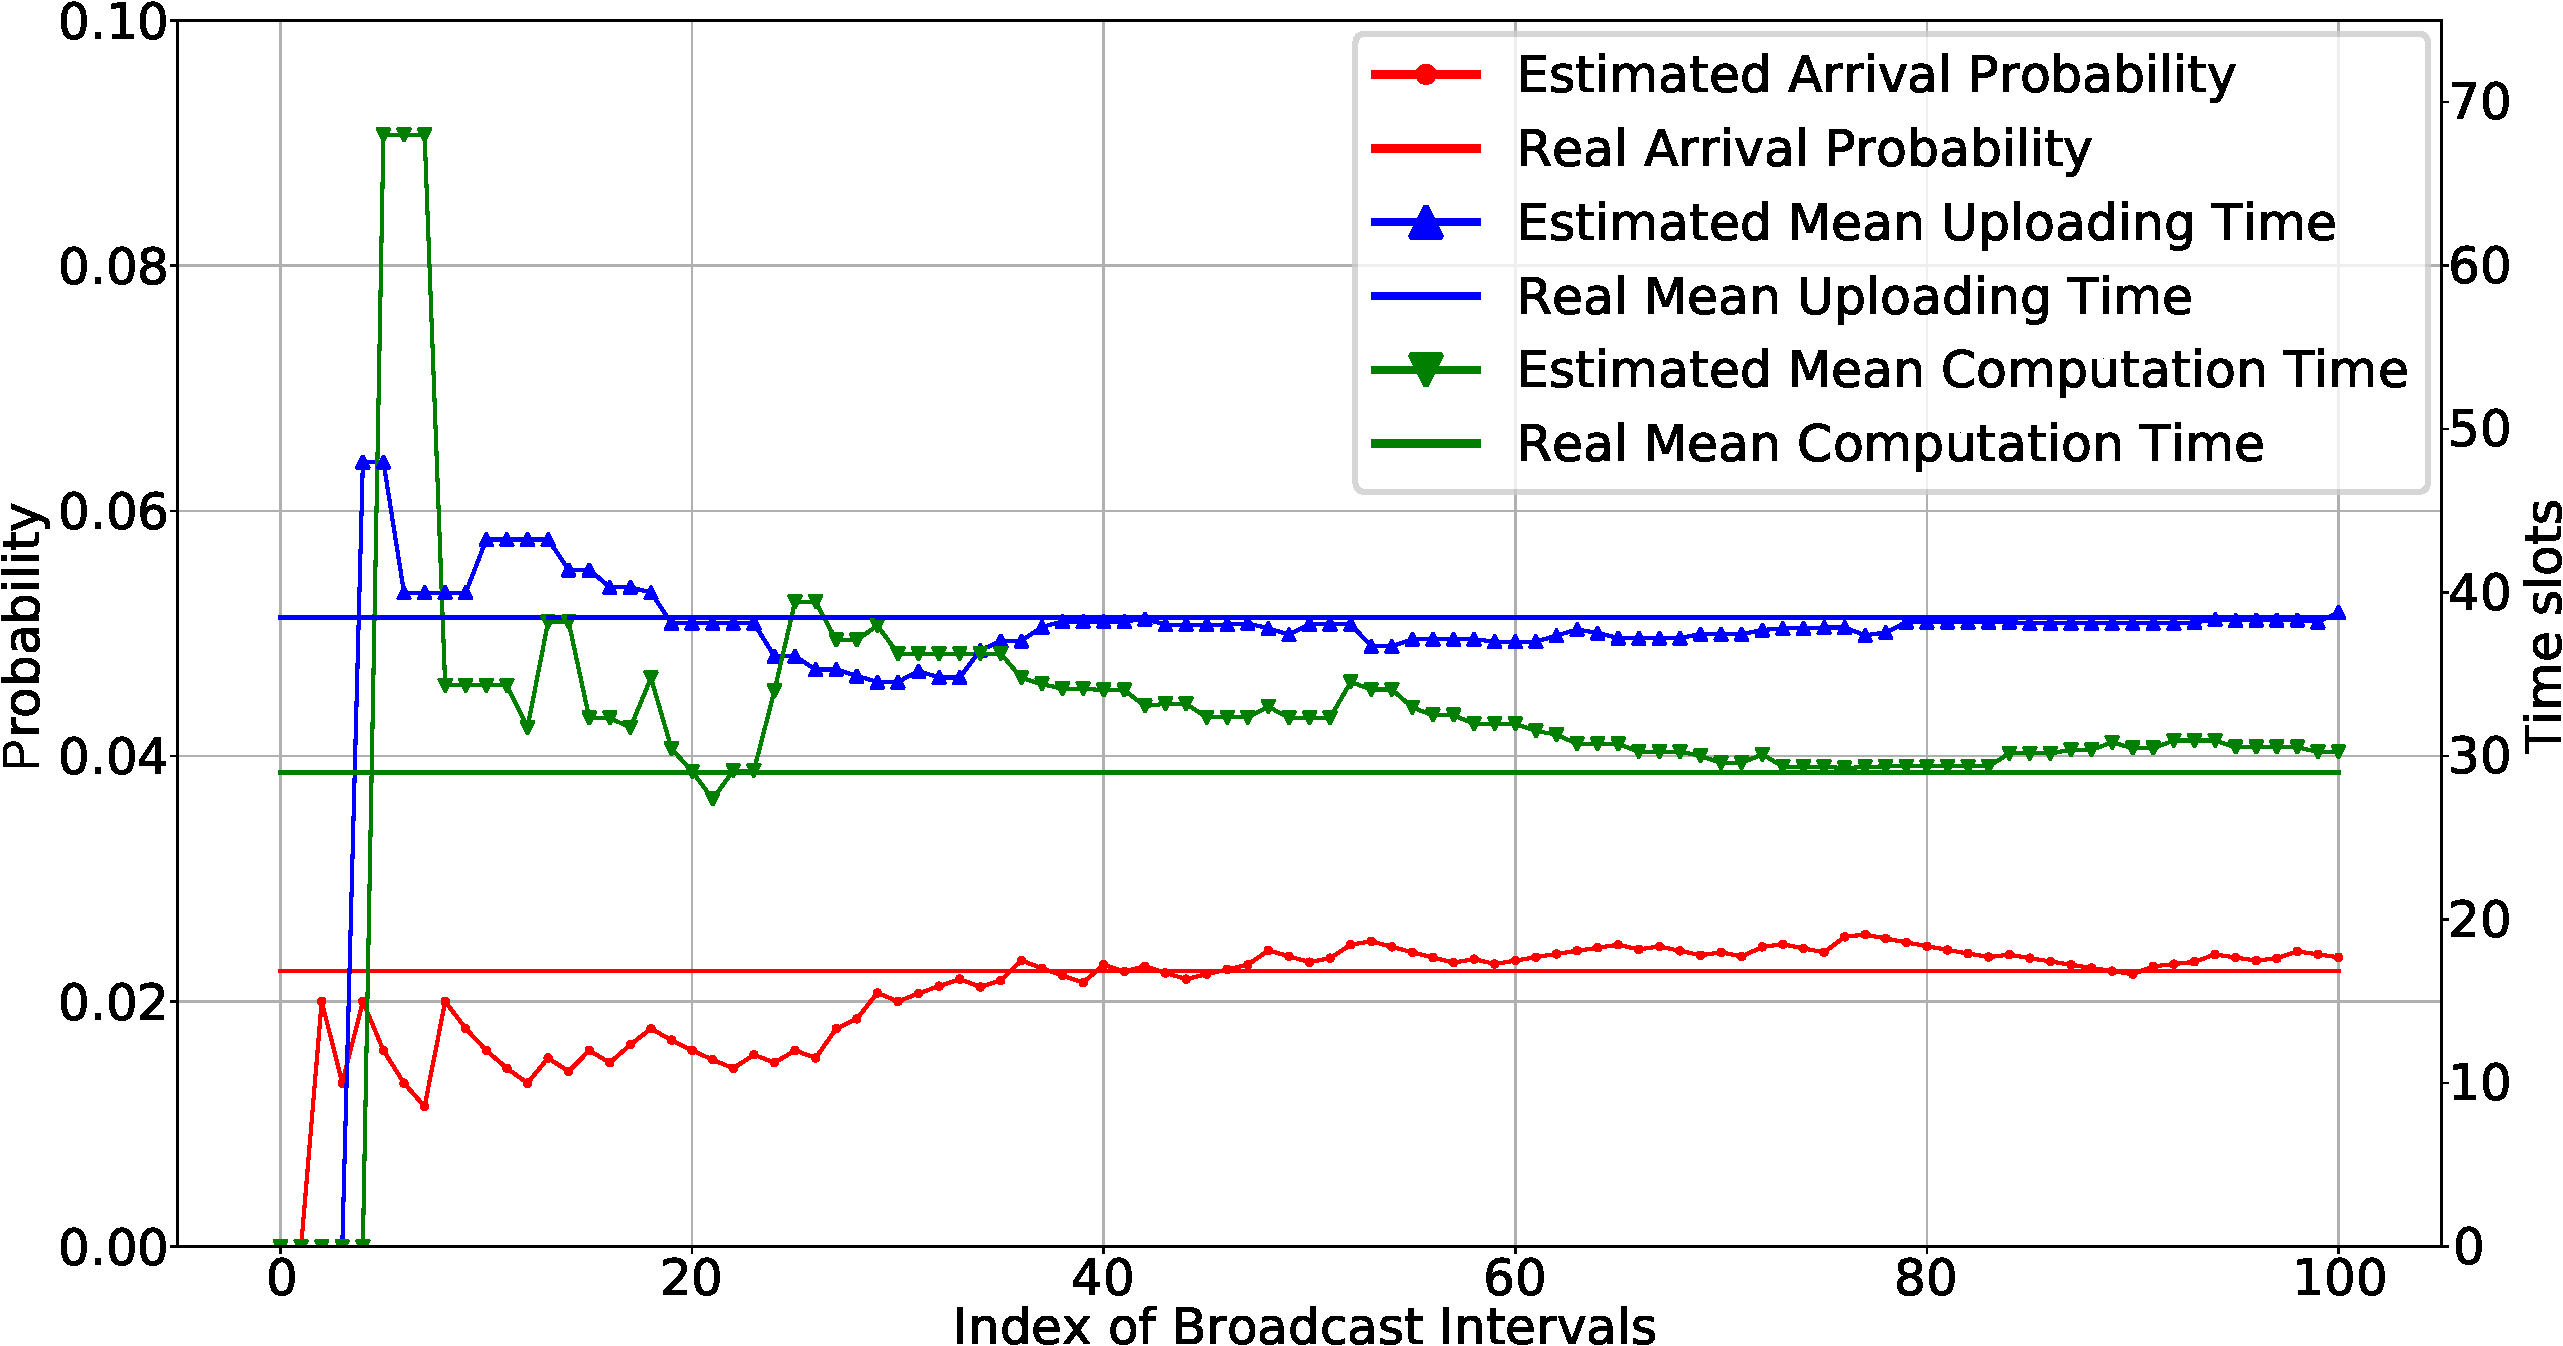
\includegraphics[width=0.45\textwidth]{the-rl-fitting.pdf}
    \caption{Illustration of reinforcement learning algorithm.} 
    \label{fig:rl_plot}
\end{figure}

\subsection{Sensitivity Study}
\label{subsec:advance}
%-----------------------------------------------------------------------------------%
\begin{figure*}[ht!]                                                                %
    \centering                                                                      %
    \begin{minipage}[b]{0.30\textwidth}                                             %
        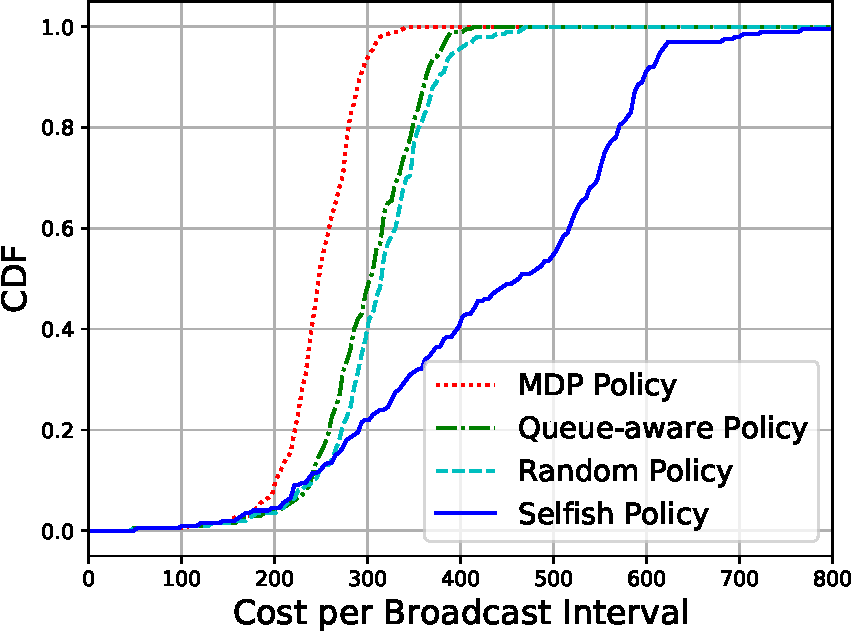
\includegraphics[width=\textwidth]{the-delay-small.pdf} \\              %
        {(a) \brlatency~as $5$ time slots.}                                              %
        \\ %NOTE: extra filling line                                                %
    \end{minipage}                                                                  %
    \begin{minipage}[b]{0.30\textwidth}                                             %
        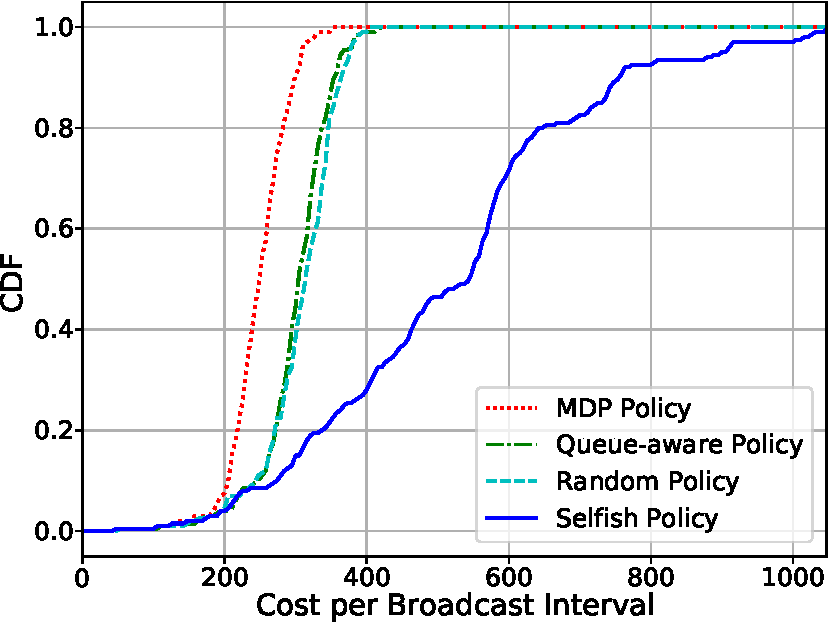
\includegraphics[width=\textwidth]{the-delay-medium.pdf} \\             %
        {(b) \brlatency~as $12$ time slots.}           %
    \end{minipage}                                                                  %
    \begin{minipage}[b]{0.30\textwidth}                                             %
        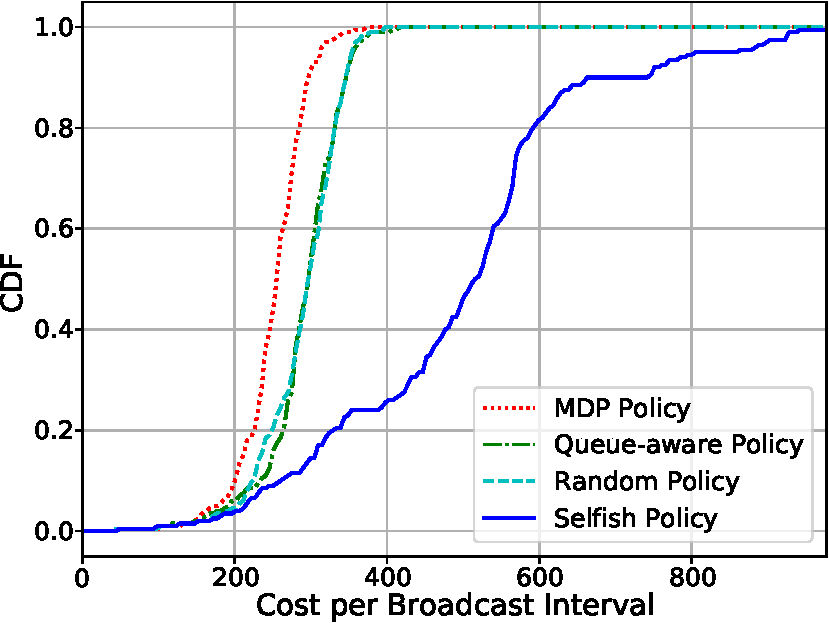
\includegraphics[width=\textwidth]{the-delay-large.pdf} \\               %
        {(c) Fixed \brlatency~as $25$}             %
    \end{minipage}                                                                  %
    \caption{Algorithm Robustness versus various signaling latency.}                %
    \label{fig:ss_signal}                                                           %
\end{figure*}                                                                       %
%-----------------------------------------------------------------------------------%


%-------------------------------------------------------------------%
\begin{figure}[hbt]                                                 %
    \centering                                                      %
    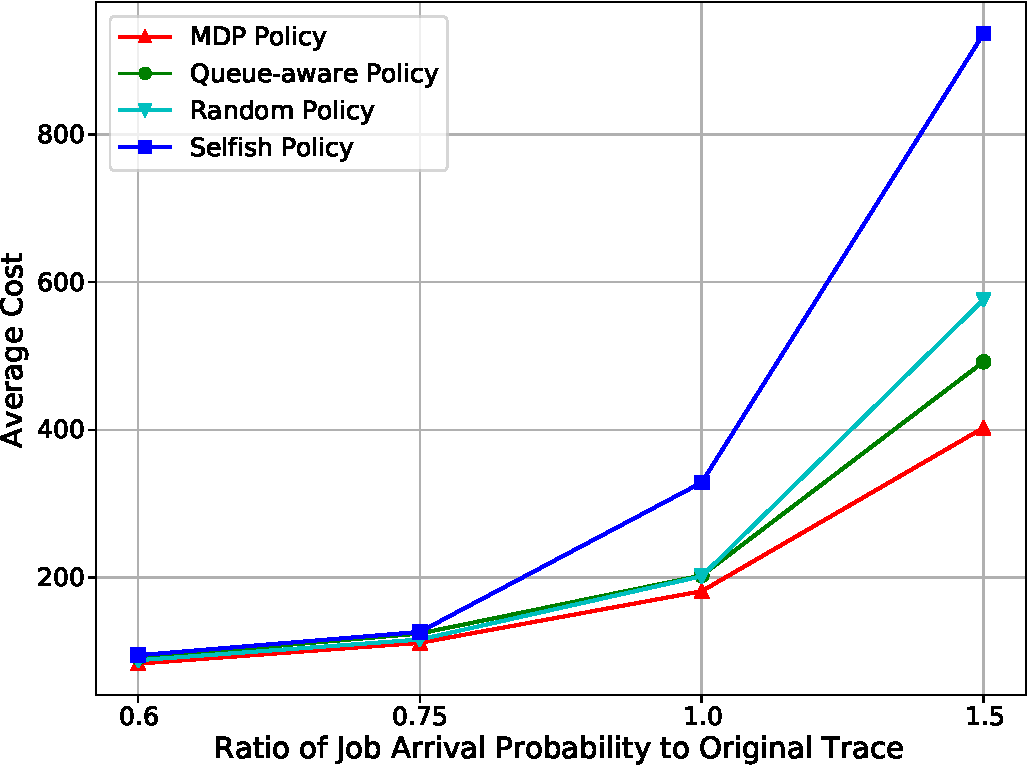
\includegraphics[width=0.45\textwidth]{the-arrival-study.pdf}   %
    \caption{Illustration of average system cost versus job arrival intensity.}
    \label{fig:ss_scale}                                            %
\end{figure}                                                        %
%-------------------------------------------------------------------%

%-------------------------------------------------------------------%
\begin{figure}[hbt]                                                 %
    \centering                                                      %
    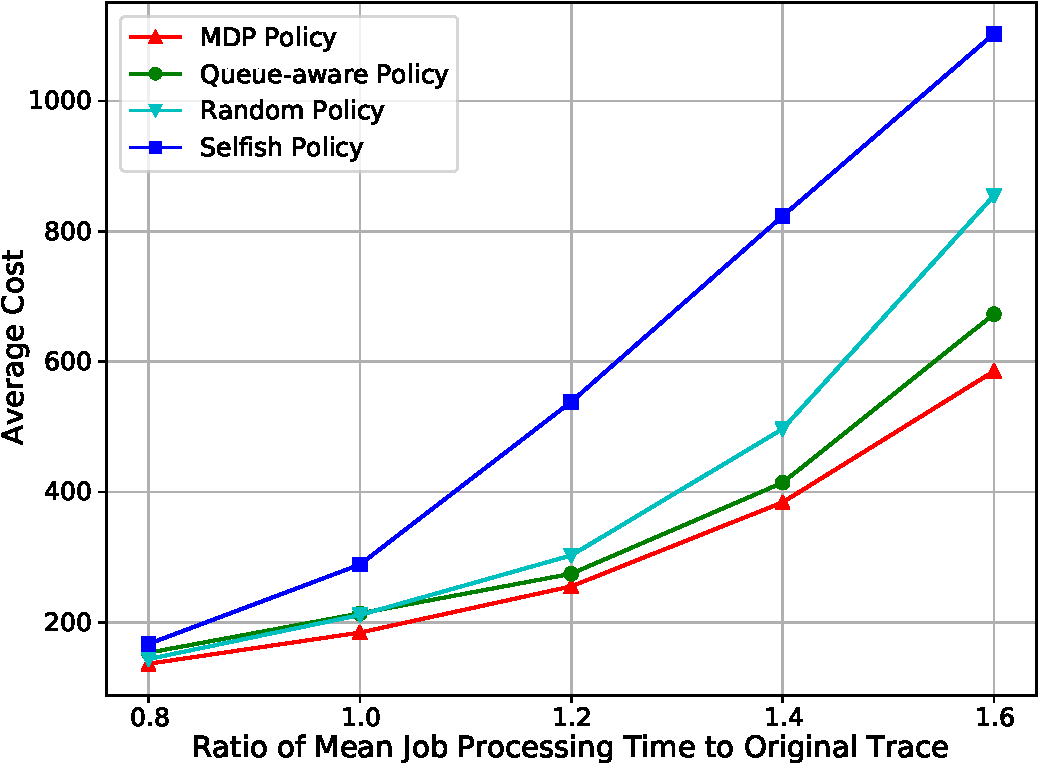
\includegraphics[width=0.45\textwidth]{the-proc-study.pdf}      %
    \caption{Illustration of average system cost versus mean processing time.}
    \label{fig:ss_dist}                                             %
\end{figure}                                                        %
%-------------------------------------------------------------------%

% %-------------------------------------------------------------------%
% \begin{figure}[hbt]                                                 %
%     \centering                                                      %
%     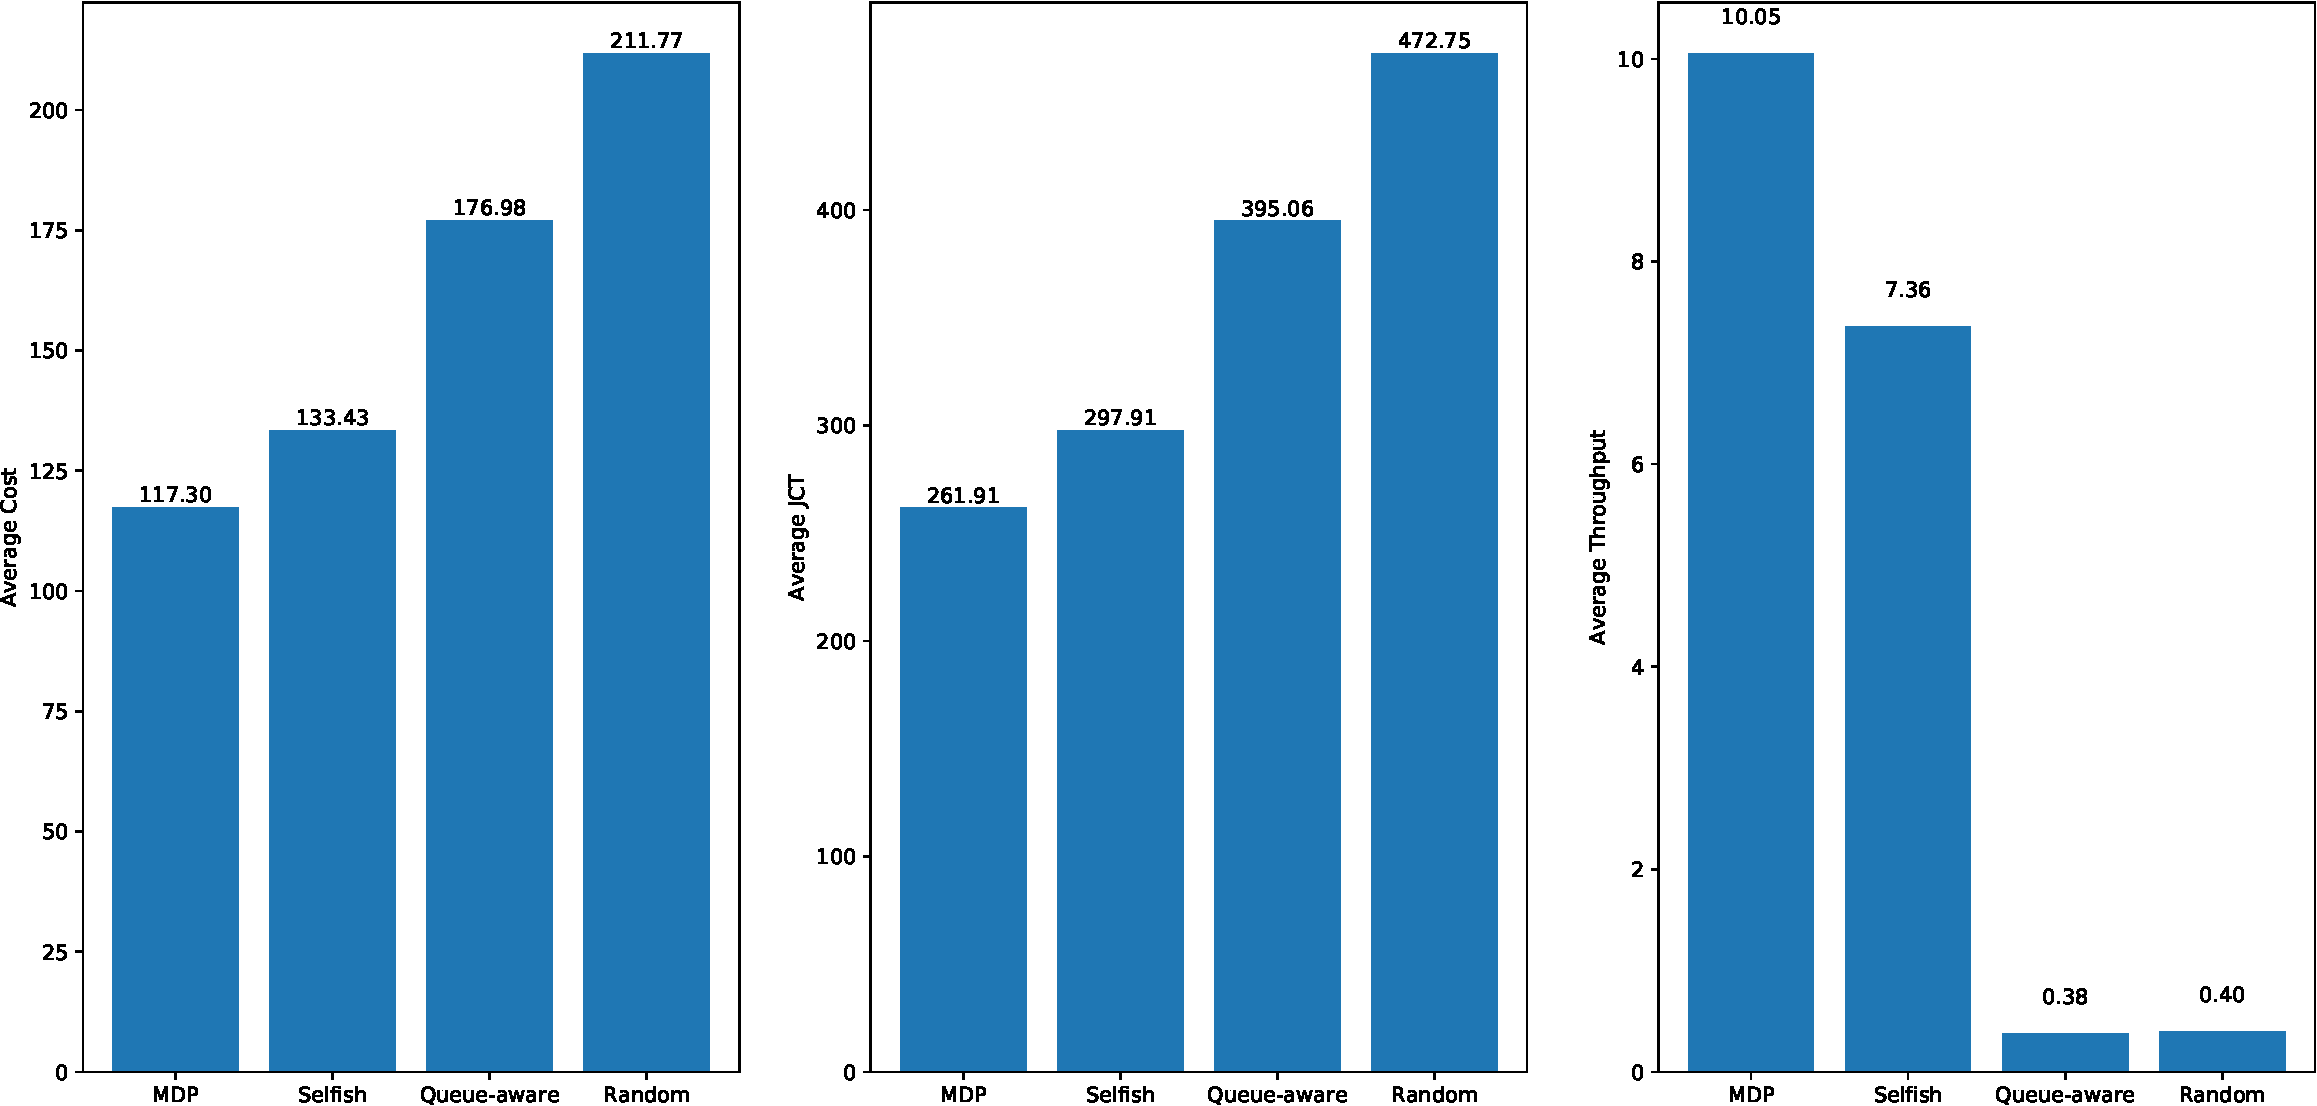
\includegraphics[width=0.45\textwidth]{bar_graph.pdf}           %
%     \caption{Illustration of impact of penalty factors on algorithms.}
%     \label{fig:ss_penalty}                                          %
% \end{figure}                                                        %
% %-------------------------------------------------------------------%

%NOTE: sensitivity study
\noindent\textbf{Signaling Latency.}
The simulation results with different \brlatency~$\mathcal{D}_{k}$ ($\forall k\in\apSet$) are illustrated in Fig.\ref{fig:ss_signal}, where the cumulative distribution function (CDF) of the job number in the system is plotted.
Specifically, the \brlatency~of all the APs is set to $5, 12, 25$ in Fig.\ref{fig:ss_signal}(a), Fig.\ref{fig:ss_signal}(b), Fig.\ref{fig:ss_signal}(c), respectively.
It can be observed from Fig.\ref{fig:ss_signal}(a) to Fig.\ref{fig:ss_signal}(c) that, with the increasing of \brlatency, the performance of Queue-aware Policy becomes worse.
The Queue-aware policy slightly outperforms the Random Policy in Fig.5(a) with smaller \brlatency~(achieving a smaller number of jobs in the system), and becomes worse in Fig.5(c) with large \brlatency.
This demonstrates that the Queue-aware Policy is sensitive to the \brlatency.
In all the figures, the proposed policy outperforms all  the benchmarks, which demonstrates its robustness versus signaling latency.
\delete{TMC-v1}{
    The simulation results with different distributions of \brlatency~$\mathcal{D}_{k}$ ($\forall k\in\apSet$) are illustrated in Fig.\ref{fig:ss_signal}, where the cumulative distribution function (CDF) of the job number in the system is plotted.
    Specifically, the \brlatency~of all the APs is set to zero and $20$ time slots in Fig.\ref{fig:ss_signal}(a) and Fig.\ref{fig:ss_signal}(c), respectively, and the \brlatency~is a random variable with integer support from $10$ to $16$ time slots in Fig.\ref{fig:ss_signal}(b).
    It can be observed from Fig.\ref{fig:ss_signal}(a) and Fig.\ref{fig:ss_signal}(c) that, with the increasing \brlatency, the performance of Queue-aware Policy becomes worse.
    It outperforms Random Policy in Fig.5(a) with zero \brlatency~(achieving a smaller number of jobs in the system), and becomes worse in Fig.5(c) with large \brlatency.
    This demonstrates that the Queue-aware Policy is sensitive to the \brlatency.
    In all the figures, the proposed policy performs better than the benchmarks, which demonstrates the robustness of its performance versus signaling latency.
}

\noindent\textbf{Job Arrival Intensity.}
We carry out the sensitivity study of job arrival intensity by integer scaling the interval of jobs arriving in Google cluster traces.
% The simulation results of various arrival intensity are illustrated in Fig.\ref{fig:ss_scale}.
The average system cost versus the number of APs is illustrated in Fig.\ref{fig:ss_scale}.
With the increasing of job arrival intensity, the average system cost increases in all the benchmarks and our proposed policy.
It can be observed that our policy performs the best.
Moreover, the performance gain becomes significant when the computation load is heavy.
This demonstrates the dispatching efficiency of the proposed policy with heavy load.
The gain is negligible for light load, where the computation capability is sufficient and dispatcher optimization may not be necessary.
\delete{TMC-v1}{
    The average system cost versus the number of APs is illustrated in Fig.\ref{fig:ss_scale}.
    With the increasing AP numbers, the average system cost increases in all the benchmarks and our proposed policy.
    It can be observed that the proposed policy has better performance than the benchmarks for all numbers of APs.
    Moreover, the performance gain becomes significant when the computation load is heavy ($K$ is large).
    This demonstrates the dispatching efficiency of the proposed policy with heavy load.
    On the other hand, the gain is negligible for light load ($K=3$), where the computation capability is sufficient and dispatcher optimization may not be necessary.
}

\noindent\textbf{Mean Processing Time.}
The simulation results of various mean processing time are illustrated in Fig.\ref{fig:ss_dist}, where the mean processing time is taken as $c_{m,j}$ of the processing time distribution $\mathbb{G}(1/c_{m,j})$ ($\forall m\in\esSet,j\in\jSpace$) in our computation model assumption.
Generally speaking, with the increasing average processing time, the average system cost increases in all the benchmarks and our proposed policy.
The simulation results are consistent with that in Fig.\ref{fig:ss_scale}.
It can be observed that the proposed policy has better performance than the benchmarks.
Moreover, the performance gain becomes significant when the computation time is long.
%(i.e., the computation load is heavy).
% On the other hand, the gain is negligible for short computation time (the computation load is light).
\delete{TMC-v1}{
    The simulation results of various distributions of processing time are illustrated in Fig.\ref{fig:ss_dist}, where the $c_{m,j}$ of the processing time distribution $\mathbb{G}(1/c_{m,j})$ ($\forall m\in\esSet,j\in\jSpace$) is generated within different ranges.
    Generally speaking, with the increasing average processing time, the average system cost increases in all the benchmarks and our proposed policy.
    The simulation results are consistent with that in Fig.\ref{fig:ss_scale}.
    It can be observed that the proposed policy has better performance than the benchmarks.
    Moreover, the performance gain becomes significant when the computation time is long (the computation load is heavy).
    On the other hand, the gain is negligible for short computation time (the computation load is light).
}

%----------------------------------------------------------------------------------------%
\delete{v20}{
    The CDF of cost is illustrated in Fig.\ref{fig:cdf_cost} where the cost of \emph{SQF policy} is nearly the same as the \emph{selfish policy}, however, the \emph{SQF policy} actually have very poor job departure rate (, throughput) compared with the other's.
    This is because the broadcast information is periodically and outdated, and SQF could not handle the penalty brought by job rejection properly.
    And we take \emph{CDF of number of jobs} other than \emph{CDF of cost} which could better reflect the performance of the average JCT target in the simulation when job rejection considered.
}
\delete{v20.2}{
    As illustrated in Fig.\ref{fig:general_timeline}, the simulation results straightly show that the proposed algorithm outperforms other benchmarks all the time with less pending jobs in the system, and the system converges fast from the start of the time.
    The detailed analysis is provided in Fig.\ref{fig:bar_plot} where three metrics are taken to demonstrate different profiles of the benchmarks.
    Firstly, the \emph{average cost} in Fig.\ref{fig:bar_plot}(a) shows that the proposed algorithm collects less cost than other algorithms within the same time duration.
    % Moreover, 
    Secondly, the \emph{average JCT} of all the jobs in Fig.\ref{fig:bar_plot}(b) resembles the shape of Fig.\ref{fig:bar_plot}(a) which proves the correctness of the cost function selection.
    Finally, The \emph{average throughput} in Fig.\ref{fig:bar_plot}(c) is defined as the division of the total number of computed jobs (i.e., the jobs being accepted by edge servers and finishing the computation) over the time duration, and the results show that the proposed algorithm have the most of jobs computed in the system.
}
%----------------------------------------------------------------------------------------%
    \section{Conclusion}
\label{sec:conclusion}
In this paper, we consider a distributed and asynchronous job dispatching design in an edge computing network residing in a MAN with multiple APs and edge servers.
The APs and edge servers periodically broadcast their local state information to facilitate distributed dispatcher design.
Due to random transmission latency, the system information observed at different dispatchers are asynchronous.
We also consider a practical scenario that not all the state information can be observed by each AP.
Hence, the distributed optimization of job dispatching strategies at all the APs is formulated as a POMDP, whose minimization objective is a discount measurement of job delivery and computation time.
We propose a novel low-complexity distributed solution framework, called \algname, based on analytical approximation of value function and one-step policy iteration, where the complicated POMDP solution or value iteration is avoided. Both the analytical and semi-analytical performance lower bounds are derived for the approximate MDP solution.
Furthremore, to handle a general scenario where the statistics of signaling latency, uploading latency and computation time are unknown in advance, an efficient online learning approach is proposed.
The simulation results show that the proposed solution framework outperforms various heuristic baselines.


    %NOTE: transition matrix and vector for AP
\appendices
\section{ Proof of Lemma \ref{lemma:w_ap} }
\label{append_1}
At the $n$-th time slot of the $t$-th broadcast interval, let $\hat{\vecG{\Theta}}^{(k,\Policy)}_{m,j}(t,n)$ denote the probability vector of job existence under dispatching policy $\Policy$, of which the explicit definition is given as follows.
\begin{align}
    \hat{\vecG{\Theta}}^{(k,\Policy)}_{m,j}(t,n) \define \Bracket{
        \hat{\theta}^{(k,\Policy)}_{m,j}(0,t,n),
        \dots,
        \hat{\theta}^{(k,\Policy)}_{m,j}(\Xi,t,n)
    },
\end{align}
where
{\small
\begin{align}
    \hat{\theta}^{(k,\Policy)}_{m,j}(\xi,t,n) \define
    \begin{cases}
        \lambda_{k,j} I[\omega_{k,j}(t)=m], &\xi=0, n < \mathcal{D}_{k}(t)
        \\
        \lambda_{k,j} I[\omega_{k,j}(t+1)=m], &\xi=0, n \geq \mathcal{D}_{k}(t) 
        \\
        \Pr\{R^{(k)}_{m,j}(\xi,t,n)=1\}, & \text{otherwise}
    \end{cases}
\end{align}
}denotes the probability that $\xi$ jobs are in uploading from the $k$-th AP to the $m$-th edge server under dispatching policy $\Policy$, at the $n$-th time slot of the $t$-th broadcast interval.
The dispatching policy $\Policy$ only affects the first entry of the probability vector, i.e., the arrival probability of one job in the time slot.
Hence, we denote the time-invariant and policy-independent transition matrix $\hat{\Gamma}^{(k)}_{m,j}$ for the state transition on AP between adjacent time slots, which is defined as follows.
\begin{align}
    \hat{\Gamma}^{(k)}_{m,j} &\define
    \begin{bmatrix}
        1 & \bar{p}^{(k)}_{m,j,0} &                       &        &                           \\
          & 0                     & \bar{p}^{(k)}_{m,j,1} &        & \text{\huge0}             \\
          &                       & \ddots                & \ddots &                           \\
          & \text{\huge0}         &                       & \ddots & \bar{p}^{(k)}_{m,j,\Xi-1} \\
          &                       &                       &        & 0                         \\
    \end{bmatrix},
\end{align}
where $\bar{p}^{(k)}_{m,j,\xi}$ denotes the probability of job still staying at the $k$-th AP in the next time slot as $\bar{p}^{(k)}_{m,j,\xi} = 1 - p^{(k)}_{m,j,\xi}$, and
\begin{align}
    p^{(k)}_{m,j,\xi} &\define \Pr\{U^{(k)}_{m,j} < (\xi+1) | U^{(k)}_{m,j}>\xi\}
\end{align}
denotes the probability of job offloading to the $m$-th edge server.

Hence, let ${\vecG{\Theta}}^{(k, \Policy)}_{m,j}(t)$ and ${\Gamma}^{(k)}_{m,j}$ denotes the probability vector and transition matrix for the adjacent broadcast intervals, respectively.
Based on the previous definitions at the scale of time slot, the expressions of $\vecG{\Theta}^{(\Policy, k)}_{m,j}(t)$ and the transition process between adjacent broadcast intervals under policy $\Policy$ are given as follows.
\begin{align}
    \vecG{\Theta}^{(k, \Policy)}_{m,j}(t) &\define \hat{\vecG{\Theta}}^{(k, \Policy)}_{m,j}(t,0),
    \\
    \vecG{\Theta}^{(k, \Policy)}_{m,j}(t+1) &= \hat{\vecG{\Theta}}^{(k, \Policy)}_{m,j}(t, \mathcal{D}_{k}(t)) \times (\hat{\Gamma}^{(k)}_{m,j})^{t_B-\mathcal{D}_{k}(t)},
    \nonumber\\
    \hat{\vecG{\Theta}}^{(k, \Policy)}_{m,j}(t, \mathcal{D}_{k}(t)) &= \vecG{\Theta}_{m,j}(t) \times (\hat{\Gamma}^{(k, \Policy)}_{m,j})^{\mathcal{D}_{k}(t)}.
\end{align}
% is composed of two-phase policy separated by $D_k(t)$, which is expressed as follows.
Given that the cost raised on APs are approximated via baseline policy $\Baseline$, the AP (saying the $k$-th AP) would adopt the same dispatching actions as $\Pi_{k}(\Stat_{k}(t), \mathcal{D}_{k}(t))$ before and after $\mathcal{D}_{k}(t)$ time slots at the $t$-th broadcast interval.
Hence, we have
\begin{align}
    \vecG{\Theta}^{(k,\Baseline)}_{m,j}(t+1) = \vecG{\Theta}^{(k,\Baseline)}_{m,j}(t) \times (\hat{\Gamma}^{(k)}_{m,j})^{t_B}.
\end{align}
and the definition of transition matrix $\Gamma^{(k)}_{m,j}$ with baseline policy $\Baseline$ as
\begin{align}
    \Gamma^{(k)}_{m,j} &\define \big( \hat{\Gamma}^{(k)}_{m,j} \big)^{t_B}.
\end{align}
Hence, the expression of the cost raised on the AP (say the $k$-th AP) under baseline policy $\Baseline$ is given as follows.
\begin{align}
    &\tilde{W}^{\AP}_{k,m,j}\Paren{\Stat(t+1)} =
    \Inorm{
        \vecG{\Theta}^{(k, \Baseline)}_{m,j}(t+1) \times
        \Bracket{
            \mat{I} - \gamma \Gamma^{(k)}_{m,j}
        }^{-1}
    }.
\end{align}


%NOTE: transition matrix and vector for ES
\section{ Proof of Lemma \ref{lemma:w_es} }
\label{append_2}
The state transition on edge server is composed of both arrival processes of all the APs in the corresponding \emph{potential AP set}, and the departure processes of jobs computation.
We first denote the offloading matrix $\bar{\Gamma}^{(k)}_{m,j}$ for the type-$j$ job offloaded from the $k$-th AP to the $m$-th edge server and the offloading probability vector $\vecG{\rho}^{(k)}_{m,j}({t,n})$ as follows, respectively ($\forall k\in\apSet, m\in\esSet_{k}, j\in\jSpace$).
\begin{align}
    \bar{\Gamma}^{(k)}_{m,j}(t,n) &\define
    \begin{bmatrix}
        0 & p^{(k)}_{m,j,0} &                 &        &                     \\
        & 0                 & p^{(k)}_{m,j,1} &        & \text{\huge0}       \\
        &                   & \ddots          & \ddots &                     \\
        & \text{\huge0}     &                 & \ddots & p^{(k)}_{m,j,\Xi-1} \\
        &                   &                 &        & 1                   \\
    \end{bmatrix},
    \\
    \vecG{\rho}^{(k, \Policy)}_{m,j}({t,n}) &\define \hat{\vecG{\Theta}}^{(k, \Policy)}_{m,j}({t,n}) \times \bar{\Gamma}^{(k)}_{m,j}.
\end{align}
However, the computational complexity of combinations of all the offloading probability vectors for the $m$-th edge server from its \emph{potential AP set} is unacceptable.
To alleviate the complexity, we rewrite the combinatorial arrival process on edge server as an equivalent Bernoulli process with \emph{small probability approximation}, i.e., there would be at most one job arriving in one time slot with the probability as the expected arrival rate of the original combinatorial distribution.
Specifically, the probability distribution of $\sum_{k\in\apSet} \vecG{\rho}^{(k, \Policy)}_{m,j}({t,n})$ is approximated as a Bernoulli distribution with the expected arrival rate denoted as $\hat{\beta}^{\Policy}_{m,j}({t,n})$ whose definition is given as
\begin{align}
    \hat{\beta}^{\Policy}_{m,j}({t,n}) &\define \sum_{k\in\apSet} \sum_{\xi=0,\dots,\Xi-1} \mathbb{E}[\vecG{\rho}^{(k, \Policy)}_{m,j,\xi}({t,n})].
    \label{eqn_0}
\end{align}

%NOTE: transition matrix and vector for Edge Server
Let $\hat{\vecG{\nu}}_{m,j}(t,n)$ denote the probability vector of $Q_{m,j}(t,n)$ at the $n$-th time slot of the $t$-th broadcast interval ($\forall m\in\esSet, j\in\jSpace$)
{\small
\begin{align}
    \vecG{\nu}_{m,j}(t,n) \define \Bracket{
        \Pr\{Q_{m,j}(t,n)=0\}, \dots, \Pr\{Q_{m,j}(t,n)=L_{max}\}
    }.
\end{align}
}The transition matrix $\hat{\mat{P}}_{m,j}(\hat{\beta}^{\Policy}_{m,j}(t,n))$ for adjacent time slots is determined by $\hat{\beta}^{\Policy}_{m,j}(t,n)$ under policy $\Policy$, whose entries are elaborated as follows.
{\small
\begin{align}
    &\Bracket{ \hat{\mat{P}}_{m,j}(\hat{\beta}^{\Policy}_{m,j}(t,n)) }_{a,b} =
    \nonumber\\
    &\begin{cases}
        (1/c_{m,j})(1-\hat{\beta}^{\Policy}_{m,j}(t,n)), & b=a-1 \\
        (1-1/c_{m,j})\hat{\beta}^{\Policy}_{m,j}(t,n), & b=a+1 \\
        (1/c_{m,j})\hat{\beta}^{\Policy}_{m,j}(t,n) + (1-1/c_{m,j})(1-\hat{\beta}^{\Policy}_{m,j}(t,n)), & a=b \\
        0, &\text{otherwise}
    \end{cases}.
\end{align}
}

Hence, let $\vecG{\nu}_{m,j}(t)$ and $\mat{P}^{\Policy}_{m,j}(t)$ denote the probability vector and transition matrix for adjacent broadcast intervals, respectively.
Based on the previous definitions in the time slot, the explicit definition is given as
\begin{align}
    \vecG{\nu}_{m,j}(t) &\define \hat{\vecG{\nu}}_{m,j}(t,0)
    \\
    \mat{P}^{\Policy}_{m,j}(t) &\define \prod_{n=0,\dots,t_B-1} \hat{\mat{P}}_{m,j}(\hat{\beta}^{\Policy}_{m,j}(t,n)),
    \\
    \vecG{\nu}_{m,j}(t+1) &= \vecG{\nu}_{m,j}(t) \times \mat{P}^{\Policy}_{m,j}(t)
\end{align}

Given that the cost raised on edge servers is approximated with baseline policy $\Baseline$, the transition matrix for state transition is affected by the baseline policy and the system states of APs which could not be decoupled.
\begin{align}
    \mathbb{E}^{\Baseline}[ Q_{m,j}({t+i+1}) | \Stat(t+i)] &\define
        \vecG{\nu}_{m,j}(t) \mat{P}^{\Baseline}_{m,j}(t+i) \vec{h}',
\end{align}
where $\vecG{h} \define [0,1,\dots,L_{max}]$.

Moreover, we notice that under the fixed baseline policy, the arrival process on edge servers would be stationary after the maximum uploading latency from the initial interval and thus the transition matrix is invariant of system states of APs.
Let $\hat{\mat{P}}_{m,j}(\hat{\beta}^{\Baseline}_{m,j}(t,n))$ be the transition matrix for the stationary arrival process under baseline policy $\Baseline$ and
{\small
\begin{align}
    \beta_{m,j}(t,n) &\define \sum_{k\in\apSet} \lambda_{k,j}I[\omega_{k,j}(t)=m] \times \Pr\{ \xi<U_{k,m,j}\le\xi+1 \}
    \nonumber\\
    &= \sum_{k\in\apSet} \lambda_{k,j}I[\omega_{k,j}(t)=m]\ (\forall n),
\end{align}
}where $U_{k,m,j}$ denotes the random variable of job uploading latency (with the unit of time slot).

Let
$\mat{P}^{\Baseline}_{m,j}(t) \define \big( \hat{\mat{P}}_{m,j}(\hat{\beta}^{\Baseline}_{m,j}(t,n)) \big)^{t_B}$
denote the transition matrix under baseline policy $\Baseline$ between adjacent broadcast intervals, we could express the cost raised on edge server under baseline policy $\Baseline$ as follows.
{\small
\begin{align}
    &\tilde{W}^{\ES}_{m,j}\Paren{\Stat(t+1)}
    = \sum_{i=0,\dots,\frac{\Xi}{T}} \gamma^{i} \mathbb{E}^{\Baseline}[ Q_{m,j}({t+i+1}) ]
    \nonumber\\
    &~~~~~~~~~~~~+ \gamma^{\frac{\Xi}{T}} 
    \vecG{\nu}({t+\frac{\Xi}{T}+1})
    \Paren{
        \mat{I} - \gamma \mat{P}^{\Baseline}_{m,j}(t)
    }^{-1} \vec{g}',
\end{align}   
}
where $\vec{g}$ is the cost vector whose definition is given in equation (\ref{eqn:g_vec}).
%----------------------------------------------------------------------------------------%

\section{ Proof of Lemma \ref{lemma:bound} }
\label{append_3}
% \hongyc{(For numerical part, show the tendency until some point; For analytical part, show the following proof.)}

Since the proposed policy $\tilde{\Policy}$ is not optimal policy and $W_{\tilde{\Policy}}(\Stat)$ represents the average system cost with the proposed policy $\tilde{\Policy}$, $V(\Stat) \leq W_{\tilde{\Policy}}(\Stat)$ is straightforward.
Let 
{\small
\begin{align*}
    \Delta(t) \triangleq &
    \sum_{t'=1}^{\infty} \gamma^{t'-1}\\\nonumber
    &\mathbb{E}^{ \tilde{\Policy} } \Bracket{
        g\Paren{\Stat(t'), \tilde{\Policy}(\Stat(t'),t-1)}
        -  g\Paren{\Stat(t'), \tilde{\Policy}(\Stat(t'),t)}
    }
\end{align*}
}
denote the improvement of the $t$-th policy update.
According to Proposition 2.3.3 (a) in \cite{dp-control}, we have $\Delta(t)\geq 0$, $\forall t$.

Hence, we have
{\small
\begin{align*}
&W_{\Baseline}(\Stat)- W_{\tilde{\Policy}}(\Stat)\\
&= 
\underbrace{\sum_{t'=1}^{N} \gamma^{t'-1} \mathbb{E}^{ \tilde{\Policy} } \Bracket{
	g\Paren{\Stat(t'), \tilde{\Policy}(\Stat(t'),0)}
	- 	g\Paren{\Stat(t'), \tilde{\Policy}(\Stat(t'),t')}
}}_{\mathfrak{F}(N)}\\
&+\sum_{t'=N+1}^{+\infty} \gamma^{t'-1} \mathbb{E}^{ \tilde{\Policy} } \Bracket{
	g\Paren{\Stat(t'), \tilde{\Policy}(\Stat(t'),0)}
	- 	g\Paren{\Stat(t'), \tilde{\Policy}(\Stat(t'),t')}
}\\
&\geq \mathfrak{F}(N) + \underbrace{\sum_{t'=N+1}^{+\infty} \gamma^{t'-1} \mathbb{E}^{ \tilde{\Policy} } \Bracket{
	g\Paren{\Stat(t'), \tilde{\Policy}(\Stat(t'),0)}
	- 	g_{\max}
}}_{\mathfrak{G}(N)},
\end{align*}
}%
where $g_{\max}$ denotes the upper-bound of the per-stage cost $g(\cdot)$.
Because  $\mathfrak{F}(N)=\sum_{t=1}^{N}\gamma^{t-1}\Delta(t)\geq 0$, $\mathfrak{F}(N)$ increases as $N$ increases.
It is obvious that $\mathfrak{G}(N)$ increases as $N$ increases, and 
\begin{align*}
\lim\limits_{N\to+\infty}\mathfrak{G}(N)=0
\end{align*}
Hence, 
\begin{align*}
\exists N,\ \mbox{s.t. }\ W_{\Baseline}(\Stat)- W_{\tilde{\Policy}}(\Stat)\geq \mathfrak{F}(N)-\mathfrak{G}(N) \geq 0.
\end{align*}

%----------------------------------------------------------------------------------------%

    % \ifCLASSOPTIONcompsoc
    %     % The Computer Society usually uses the plural form
    %     \section*{Acknowledgments}
    % \else
    %     % regular IEEE prefers the singular form
    %     \section*{Acknowledgment}
    % \fi
    % The authors would like to thank...

    \ifCLASSOPTIONcaptionsoff
        \newpage
    \fi

    \bibliographystyle{IEEEtrans}
    \bibliography{references/final.bib}

    
\vspace{-0.3cm}
\begin{IEEEbiography}[{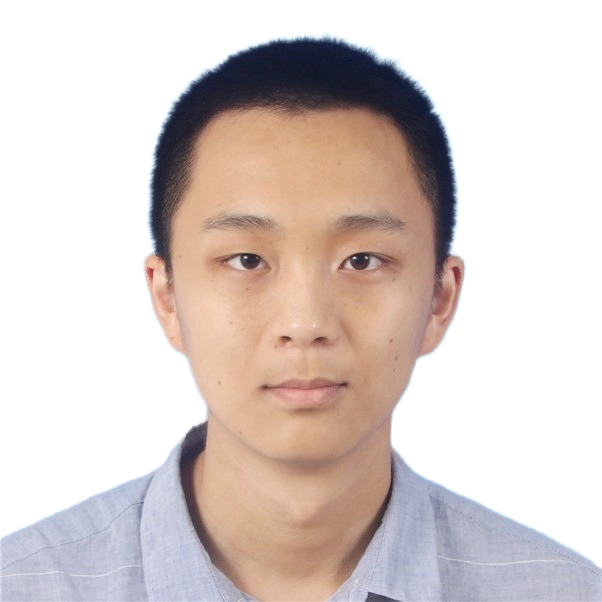
\includegraphics[width=1in,height=1.25in,clip,keepaspectratio]{images/photo/hong.png}}]{Yuncong Hong}
    received his B.ENG degree in electrical and electronic engineering from Southern University of Science and Technology of China (SUSTech) in 2018. He is currently in a joint Ph.D program in computer science with the University of Hong Kong (HKU) and SUSTech. He is co-supervised by Prof. Francis Lau and Prof. Rui WANG. His research interests include edge computing, approximation MDP and online learning.
\end{IEEEbiography}
\vspace{-1cm}

\begin{IEEEbiography}[{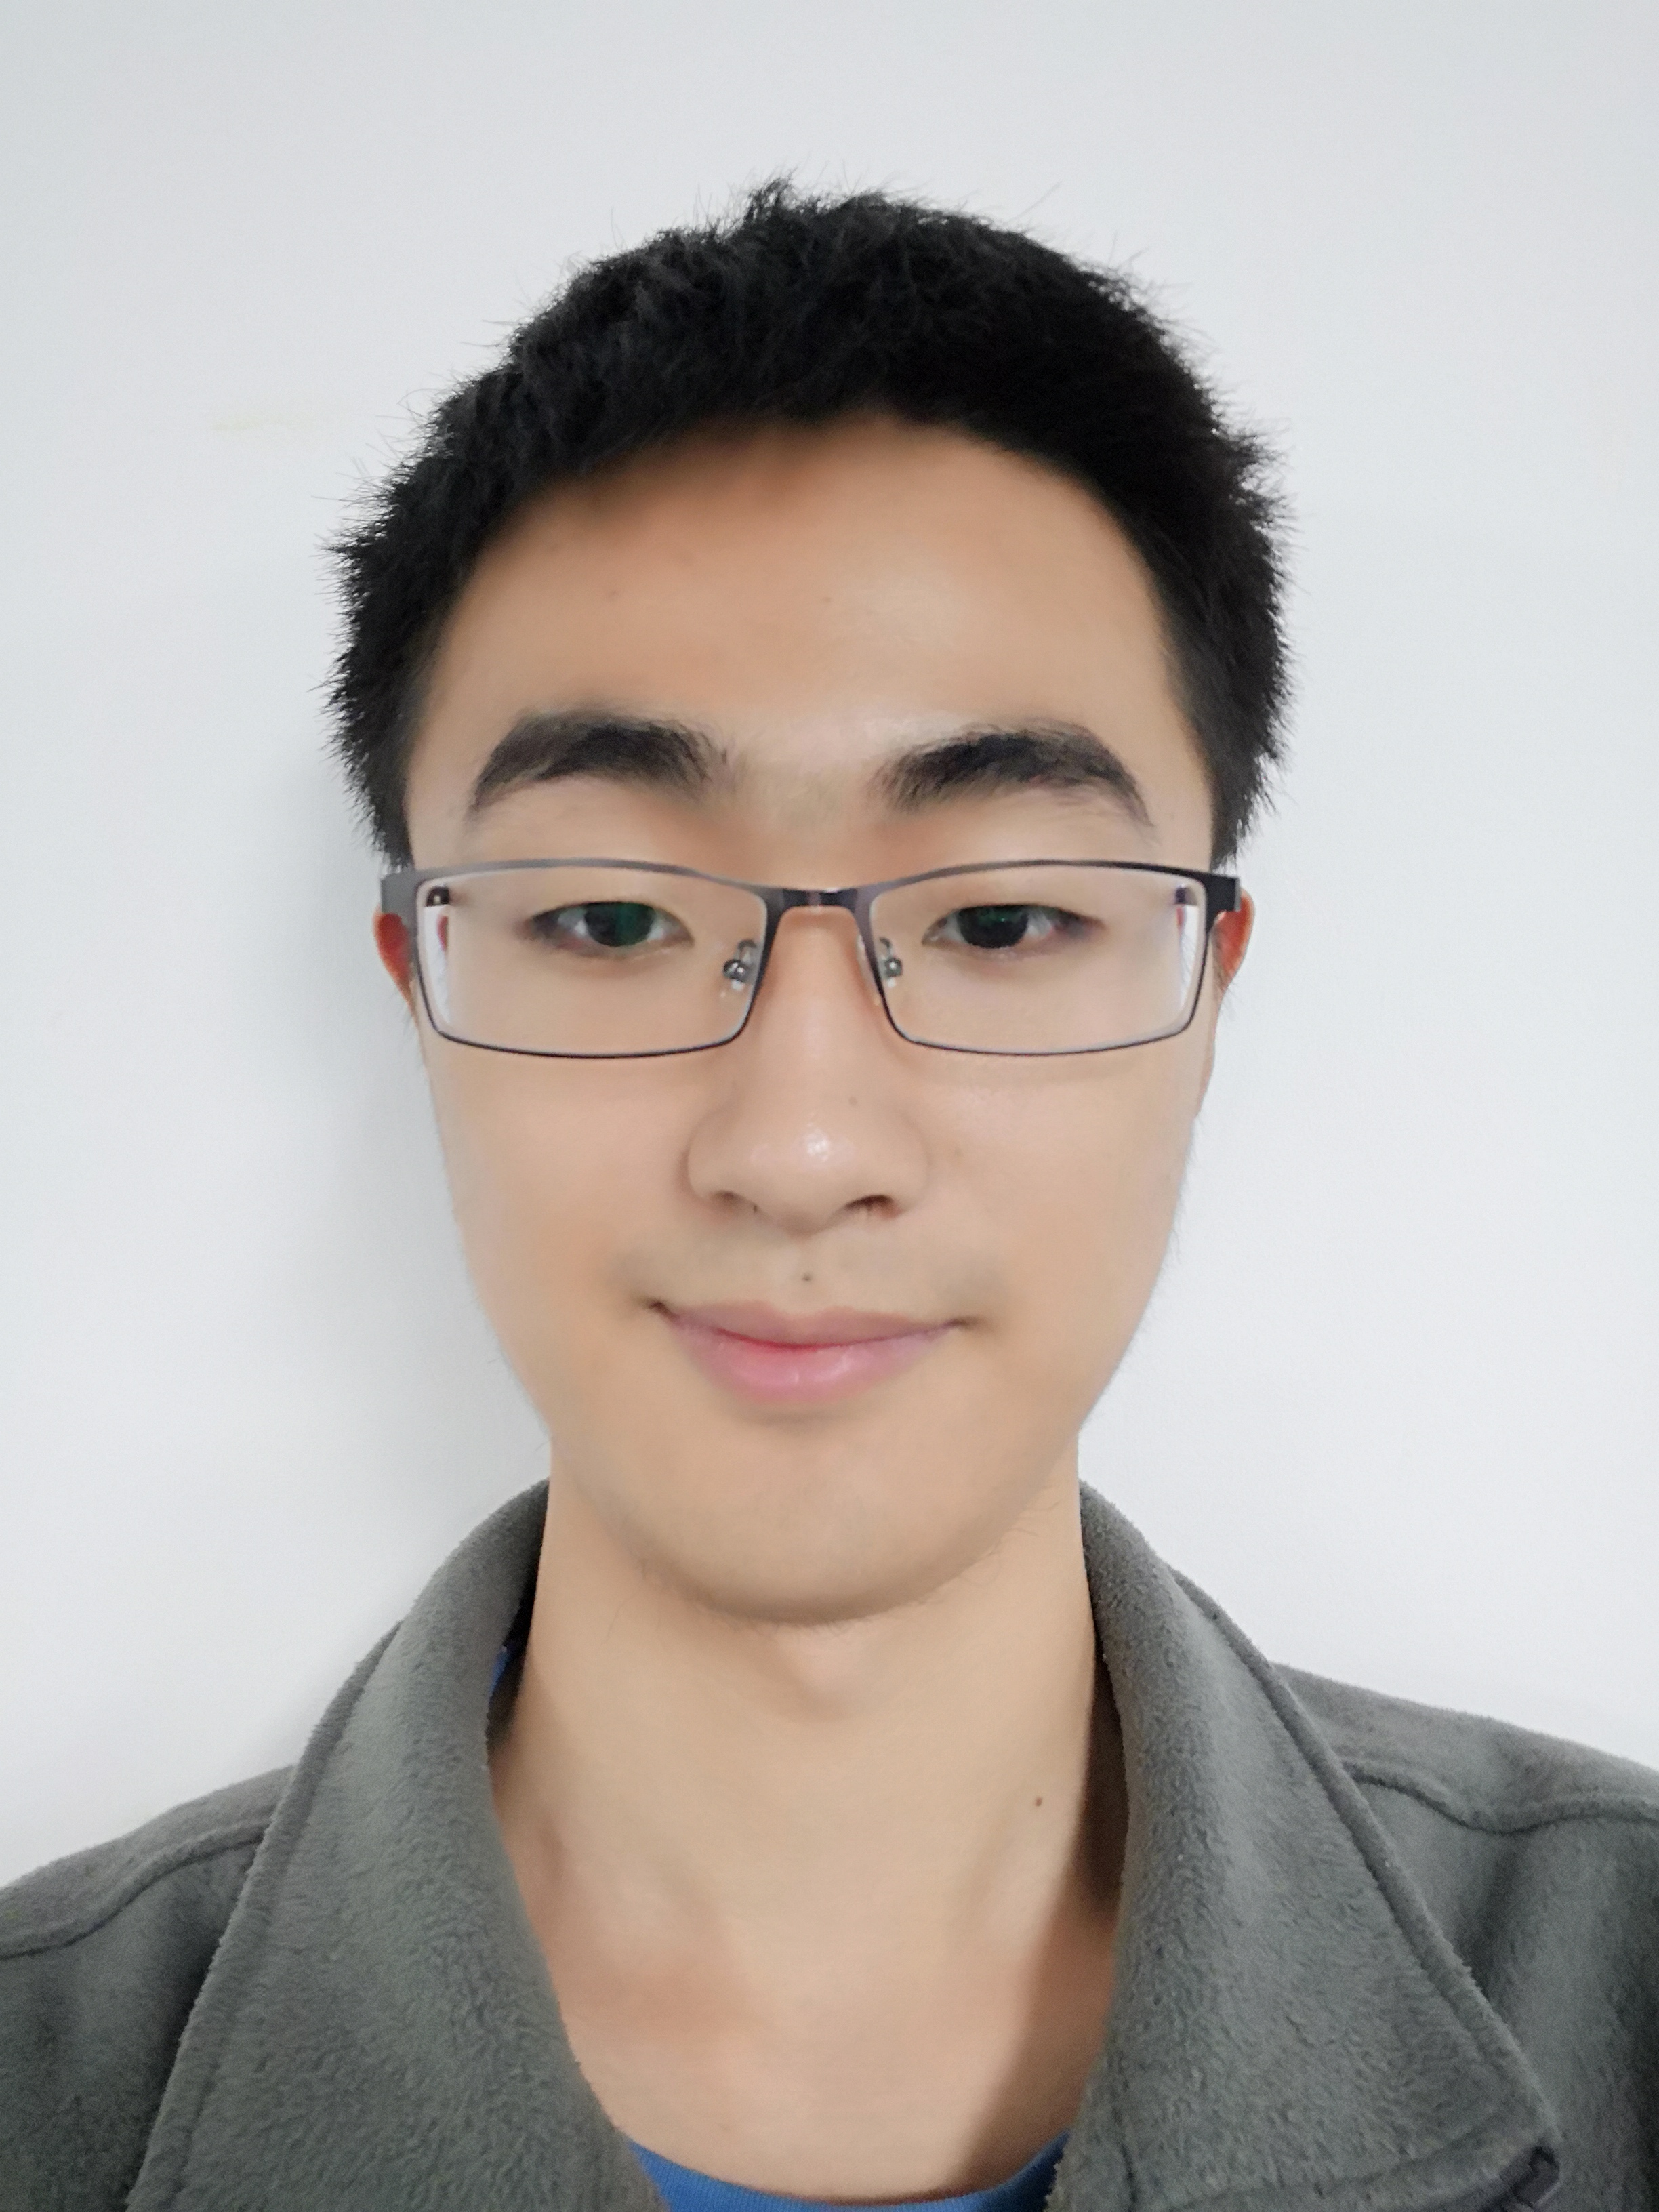
\includegraphics[width=1in,height=1.25in,clip,keepaspectratio]{images/photo/lv.jpg}}]{Bojie Lv}
    (S'18) received the B.E. degree in Communication Engineering from the Southern University of Science and Technology (SUSTech) in 2018, and MPhil degree (ranked top 2) from the Information and Communication Engineering from Harbin Institute of Technology (HIT) in 2020. He is now pursuing the math PhD degree in SUSTech. His research interests are in the area of stochastic optimization and resource allocation in the wireless networks.
\end{IEEEbiography}
\vspace{-1cm}

\begin{IEEEbiography}[{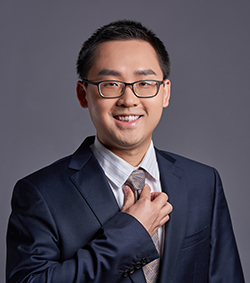
\includegraphics[width=1in,height=1.25in,clip,keepaspectratio]{images/photo/wang.jpg}}]{Rui Wang}
    received the B.S. degree from the University of Science and Technology of China in 2004 and the Ph.D. degree in wireless communications from The Hong Kong University of Science and Technology in 2008.
    From 2009 to 2012, he was a Senior Research Engineer with Huawei Technologies, Co., Ltd. Since 2012, he has been with the Southern University of Science and Technology of China, as an Associate Professor. He has research experience in both academia and industry. He has authored over 30 papers in top-level IEEE journals and flagship international conferences, especially in the area of wireless radio resource optimization and interference management. He has contributed to over 20 U.S. patent applications and over 30 Chinese patent applications (20 of them have been granted). He was also involved in the development of interference mitigation technology for 5G systems.
\end{IEEEbiography}
\vspace{-1cm}

\begin{IEEEbiography}[{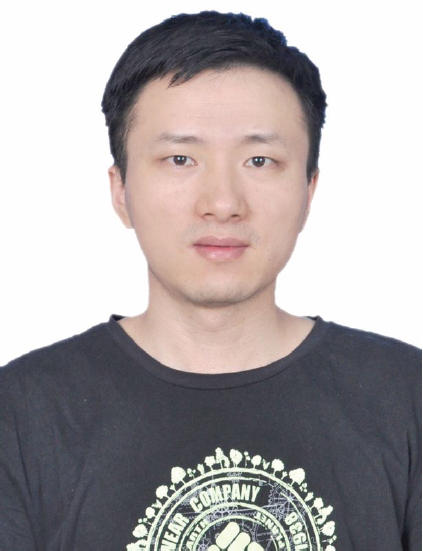
\includegraphics[width=1in,height=1.25in,clip,keepaspectratio]{images/photo/tan.png}}]{Haisheng Tan}
    received his B.E. degree in Software Engineering and B.S. degree in Management both from University of Science and Technology of China (USTC) with the highest honor. Then, he got his Ph.D. degree in computer science at the University of Hong Kong (HKU) in 2011. After that, he worked as a postdoctoral fellow in Prof. Andrew Yao's group at Tsinghua University, Beijing, China. He is currently an associate professor at USTC. His research interests include algorithms and networking. Dr. Tan has published over 50 papers in prestigious journals and conferences, mainly in the areas of wireless networking, data center networks and cloud computing. He recently received the awards of ACM China Rising Star (Hefei Chapter), and the Distinguished Member of INFOCOM 2019 TPC. He is senior member of IEEE.
\end{IEEEbiography}
\vspace{-1cm}

\begin{IEEEbiography}[{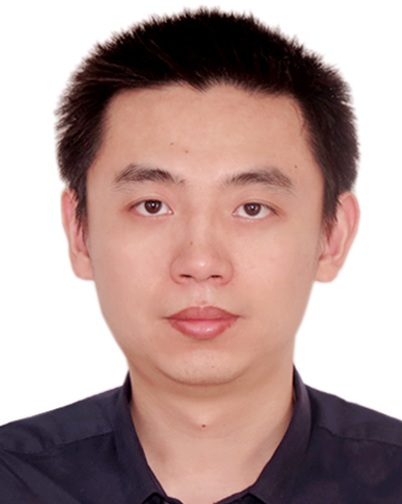
\includegraphics[width=1in,height=1.25in,clip,keepaspectratio]{images/photo/han.jpg}}]{Zhenhua Han}
    received Ph.D. in computer science from the University of Hong Kong, and B.Eng in electronic and information engineering from the University of Electronic Science and Technology of China. He is now a researcher in Microsoft Research Asia. His research interests include cloud computing, AI systems, cluster scheduling. Many of his works have been published in top venues such as USENIX OSDI, IEEE INFOCOM, and IEEE/ACM Transaction on Networking.
\end{IEEEbiography}
\vspace{-1cm}

\begin{IEEEbiography}[{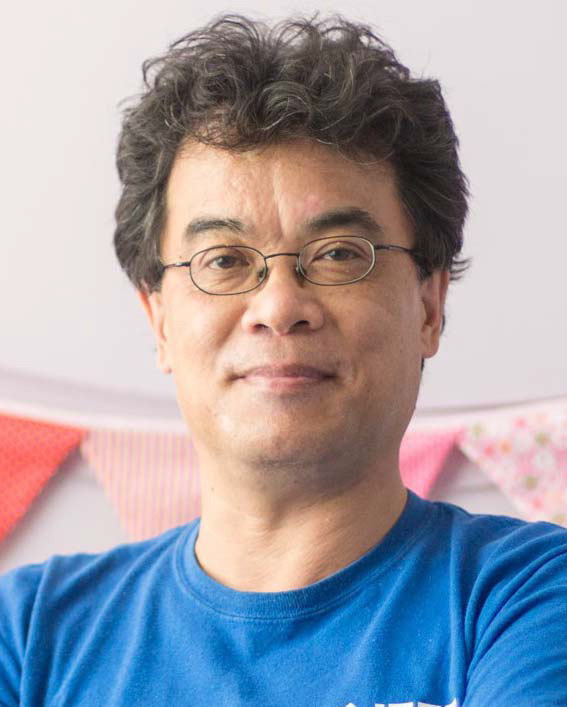
\includegraphics[width=1in,height=1.25in,clip,keepaspectratio]{images/photo/lau.png}}]{Francis~C.M.~Lau}
    received the Ph.D. degree from the Department of Computer Science, University of Waterloo. He is currently a Professor in computer science with The University of Hong Kong, China. His research interests include computer systems, networks, programming languages, and application of computing in arts. He is currently the Editor-in-Chief of the Journal of Interconnection Networks.
\end{IEEEbiography}
\vspace{-1cm}

\end{document}